% !TEX root = ../thesis.tex
\graphicspath{{Chapter2/Chapter2Figs/}{Chapter2/Chapter2Figs/}}
 
\chapter{Use Fine-TunedLarge Language Model to Generate Consistent and Sufficient Synthetic Texts}\label{ch:chapter:2}

\section{Introduction}\label{ch2:sec:introduction}  
Government announcements shows significant impacts on the interest rate market (\cite{vergote2012}, \cite{rosa2013financial}, \cite{jubinski2013fomc}. ). Meanwhile, the U.S. government bond deviates, such as the 10-Year Treasury Note futures and options, are traded almost continuously, except for a one-hour halt from 4PM to 5PM Central Time (CT). This nearly continuous trading allows traders to react to the events and press releases at any time. 

Current models for predicting the implied volatility surface (IVS),  built on the Efficiency Market Hypothesis (EMH, \cite{fama1970}), reply only on the quantitative data. For instance, parametric models, like the Heston Stochastic Volatility Model (\cite{Heston:1993}) and the Stochastic Alpha Beta Rho (SABR) Model (\cite{sabr2002}), need to be calibrated on the current shape of the surface. However, these model failed in accounting for qualitative data as a part of themselves. 

Consequently, there is pressing need for forecasting models that integrate potential qualitative information. However, Unlike the quantitative data, qualitative data are  inherently discontinuous, making historical data insufficient for analyzing diverse scenarios. For instance, the Federal Reserve has only adjusted the Fed Fund Rate 130 times since 1990s. To address this challenge, we propose utilizing a fine-tuned large language model (LLM) to generate synthetic texts across various scenarios, thereby enhancing the volatility models' ability to handle qualitative inputs effectively.


The exceptional predictive capabilities of the Artificial Neural Networks (ANNs) makes them ideal tools for synthesizing both quantitative and qualitative data. \cite{guo2024generative} conducted a comprehensive survey, describing the diverse applications of synthetic data across industries. This work addresses critical concerns such as confidentiality of data, and the augmentation of training datasets. \cite{potluru2023synthetic}, also referenced by \cite{assefa2020generating}, highlights the specific utility of the synthetic data in finance, notably its role in enhancing risk management practices within banking institutions.


Synthetic data has been accepted by the financial researchers as a powerful tool in the robustness tests. For instance, \cite{cao2022synthetic} employed a synthetic limit order book to test the performance of different forecasting models, while \cite{carvajal2022synthetic} used synthetic stock prices to train a trading model. 


Besides the time-series data, the financial industry manages a large volume of structured documents, such as the financial reports, the Minutes for the Monetary Policy Committee (MPC) meetings of the Bank of England, and the Minutes of the Federal Open Market Committee (FOMC) meetings of the Federal Reserve. 

% Meanwhile, the significant developed Large Language Model (LLM) in the Natural Language Process (NLP) 
Meanwhile, the recent remarkable developments in Neutral Networks (NNs), Large Language Models (LLMs) have been rapidly advanced and outstandingly perform in a broad range of Natural Language Processing (NLP) tasks. LLMs are pre-trained on a diverse array of texts, enabling them to generate high-quality, human-like text. Some models are fine-tuned with specific datasets for specialized tasks. The significant success of LLMs makes them ideal for generating variety of synthetic structured texts, such as labeled sentence pairs (\cite{schick2021generating}),  instruction-following data (\cite{peng2023instruction}), and news report (\cite{yu2024large}). However, generating synthetic documents remains a challengeable topic. There are limit researches have been made in finance, but several applications in other sectors, such as healthcare, where LLMs have been employed to create clinic notes (\cite{li2021synthetic}, \cite{meoni2024generating}). 

Therefore, to the best of our knowledge, our research constitutes the pioneering try to fine-tune LLMs for the generation of  consistent structured texts specifically in financial domain. 


% Additionally, sufficient information in the responses is also our concern. We employ Shapley Value ($\mathcal{SV}$) to calculate the marginal contribution of the prompts to the responses. Because we need the response to contain all the economic and financial information in the prompt. As the prompts increase, the marginal contribution should be non-negative. Therefore, the sufficient test will conduct under the null hypothesis:

% \begin{equation*}
%     H_0: \mathcal{SV} < 0
% \end{equation*}


Finally, our research aims to contribute to the exiting literature in the following aspects:
\begin{itemize}
    \item \textit{1. We introduce a novel approach for generating synthetic structured texts that span various scenarios. This innovation will assist researchers in conducting robustness tests for their models by providing almost unlimited data.}
    \item \textit{2. Our research substantiates the generative capacity of LLMs for structured texts. Consequently, other researchers can leverage our methods to fine-tune LLMs with alternative structured texts, such as firm specific reports and legal required documents, fostering broader applicability.}
    \item \textit{3. Our research translates discrete qualitative information into a continuous distribution, which offers fresh perspectives on risk management strategies within the financial sector}
\end{itemize}


Our chapter is structured as followings: Section \ref{ch2:sec:related work} will review the related works in synthetic data. Additionally, the current literature about LLM will be provided in Section \ref{ch2:sec:llm}. Following that, Section \ref{ch2:sec:the dataset} will talk about our dataset, Section \ref{ch2:sec:model finetuning} will detailed illustrate our method in model fine-tuning. Finally, Section \ref{ch2:sec:empirical results} is the empirical results of our model. 



\section{Literature Review}\label{ch2:sec:lr}

\subsection{Related Works on Synthetic Data}\label{ch2:sec:lr:related work}
Current literature on synthetic data generation has shown remarkable improvement with the significant advancement of the Generative Artificial Intelligence (AI) technologies. 

The Royal Society defined Synthetic data as \textit{`` ... data that has been generated using a purpose-built mathematical model or algorithm, with the aim of solving a (set of) data science task(s) (\cite{jordon2022synthetic}).''}  Traditional ways generating synthetic data involve numerical processes based on some assumptions and random numbers drawn from normal or uniform distributions, such as the Autoregressive Moving Average model (ARMA, \cite{whittle1951hypothesis}) and the Generalized AutoRegressive Conditional Heteroskedasticity Model (GARCH, \cite{Bollerslev:1986}). However, the remarkable development in Artificial Neutral Network (ANN) provides novel approaches in generating synthetic data. These models are pre-trained on the exiting data, which can help the models capture various features of the data. 

% distribution
\cite{athey2021using} were among the first to introduce the Wasserstein Generative Adversarial Network (WGAN, \cite{arjovsky2017wasserstein} and \cite{goodfellow2020generative}) as a powerful tool for generating synthetic economic data with the similar distribution of the raw data. They utilized this technique to replace the conventional Monte Carlo Simulation in testing robustness of economic models. Subsequently, \cite{kaji2023adversarial} integrated structured models with the WGAN to effectively model complex distributions.  

% time series
Regarding time-series data, the Long Short-Term Memory (LSTM, \cite{hochreiter1997long}) has gained widespread popularity. For instance, \cite{carvajal2022synthetic} applied the LSTM to model stock price dynamics. \cite{fischer2018deep} used the model for forecasting the S\&P 500 index, while \cite{liu2019novel} employed it to predict the volatility of the S\&P 500 index. 

% texts
Finally, Large Language Models (LLMs) have recently been harnessed across a broad spectrum of Natural Language Processing (NLP) tasks. Current literature indicates LLMs serve as a formidable resource for generating human-like texts, significantly advancing the field of NLP. \cite{potluru2023synthetic}, \cite{assefa2020generating}, and \cite{guo2024generative} offer a survey listing applications and challenges associated with employing LLMs for synthesizing text data. 

In the financial domain, documents, such as prospectus, credit reports, purchase orders, sustainability disclosures, and income statements, are presented in a range of required formats and encompass a diversity of semantics. Analyzing these documents can provide critical insights into risk management for firms, banks and governments. However, curating these documents presents significant challenges, especially when they are proprietary or subject by copyright and licensing restrictions. Synthetically generated documents provide a viable alternative and cheap way to the explicit collection of documents.


\subsection{Large Language Models (LLM) for text generation}\label{ch2:sec:lr:llm}
A large number of researches in Natural Language Processing (NLP) involves forecasting the following words given some sequences. The main idea is to choose the words with the highest score given the current contexts:


\begin{equation*}
    w_{i+1}^* = \underset{w_{i+1}}{arg\,max}\,f(w_{i+1} | w_1, w_2, ...,w_i; Context)
\end{equation*}

where $\bm{w} = w_1, w_2, ..., w_{i}$ is a sequence of words, $f(\cdot)$ is a parameterized model. Therefore, the key in NLP is to find the ``right'' $w_{i+1}$ or the ``right'' quantitative measure of $w_{i+1}$. \cite{mikolov-etal2013} firstly proposed a ``Word2Vec'' model which can compute the vector representation of a word using a Neural Network. Moreover, considering that a single word may have different meanings in different contexts, \cite{peter-etal2018} enhances the word vector by incorporating linguistic contexts using Bi-directional LSTM. However, there two challenges with the traditional architectures, such as the CNN, RNN, and LSTM. Firstly, with the length of the sequences increasing, the earlier contexts may be lost. This is a common issue with neural networks where information accumulates exponentially. If the coefficient in $f(\cdot)$ is less than 1 and n becomes very large, the earlier information (e.g. $h_1(\cdot)$ in Fig. \ref{fig: ch0: rnn.png}) becomes too diluted to effectively influence the prediction. This diminishing effect of earlier data points is particularly problematic in long sentences, where critical contextual information may be lost. Additionally, eue to their reliance on sequential data, these models cannot process each word in parallel. This sequential dependency limits the speed of processing, as each word or piece of information must be processed one after the other, rather than simultaneously.

To address these issues, \cite{bahdanau-etal2014} pioneered the use of ``attention" by integrating a weight into the word vector. The underlying concept is to assign a lower weight to less significant words, thereby enhancing the model's focus on more relevant information. Following this, \cite{cheng-etal2016} introduced a mechanism known as intra-attention (or self-attention) in machine reading. This approach generates attention weights based on the words within in the current sentence (or sequence), allowing for a nuanced understanding of text. \cite{vaswani-etal2018} introduced a framework named "Transformer", which distinguishes itself from previously mentioned models by being entirely based on the concept of self-attention, eschewing traditional architectures like CNNs, RNNs, or LSTMs. Because the self-attention mechanism allows us to calculate the weights for all the words in a sequence simultaneously, the computation in the Transformer can be parallelized This significantly reduces the time cost.

The Transformer consists of two main components, Encoder and Decoder. The Encoder (Fig. \ref{fig: ch0: transformer_encoder}) is used to create accurate word vectors incorporating the position information and the context information. The Decoder (Fig. \ref{fig: ch0: transformer_decoder}) will predict the next words based on the input sequences.


\begin{figure}[h]
    \centering
    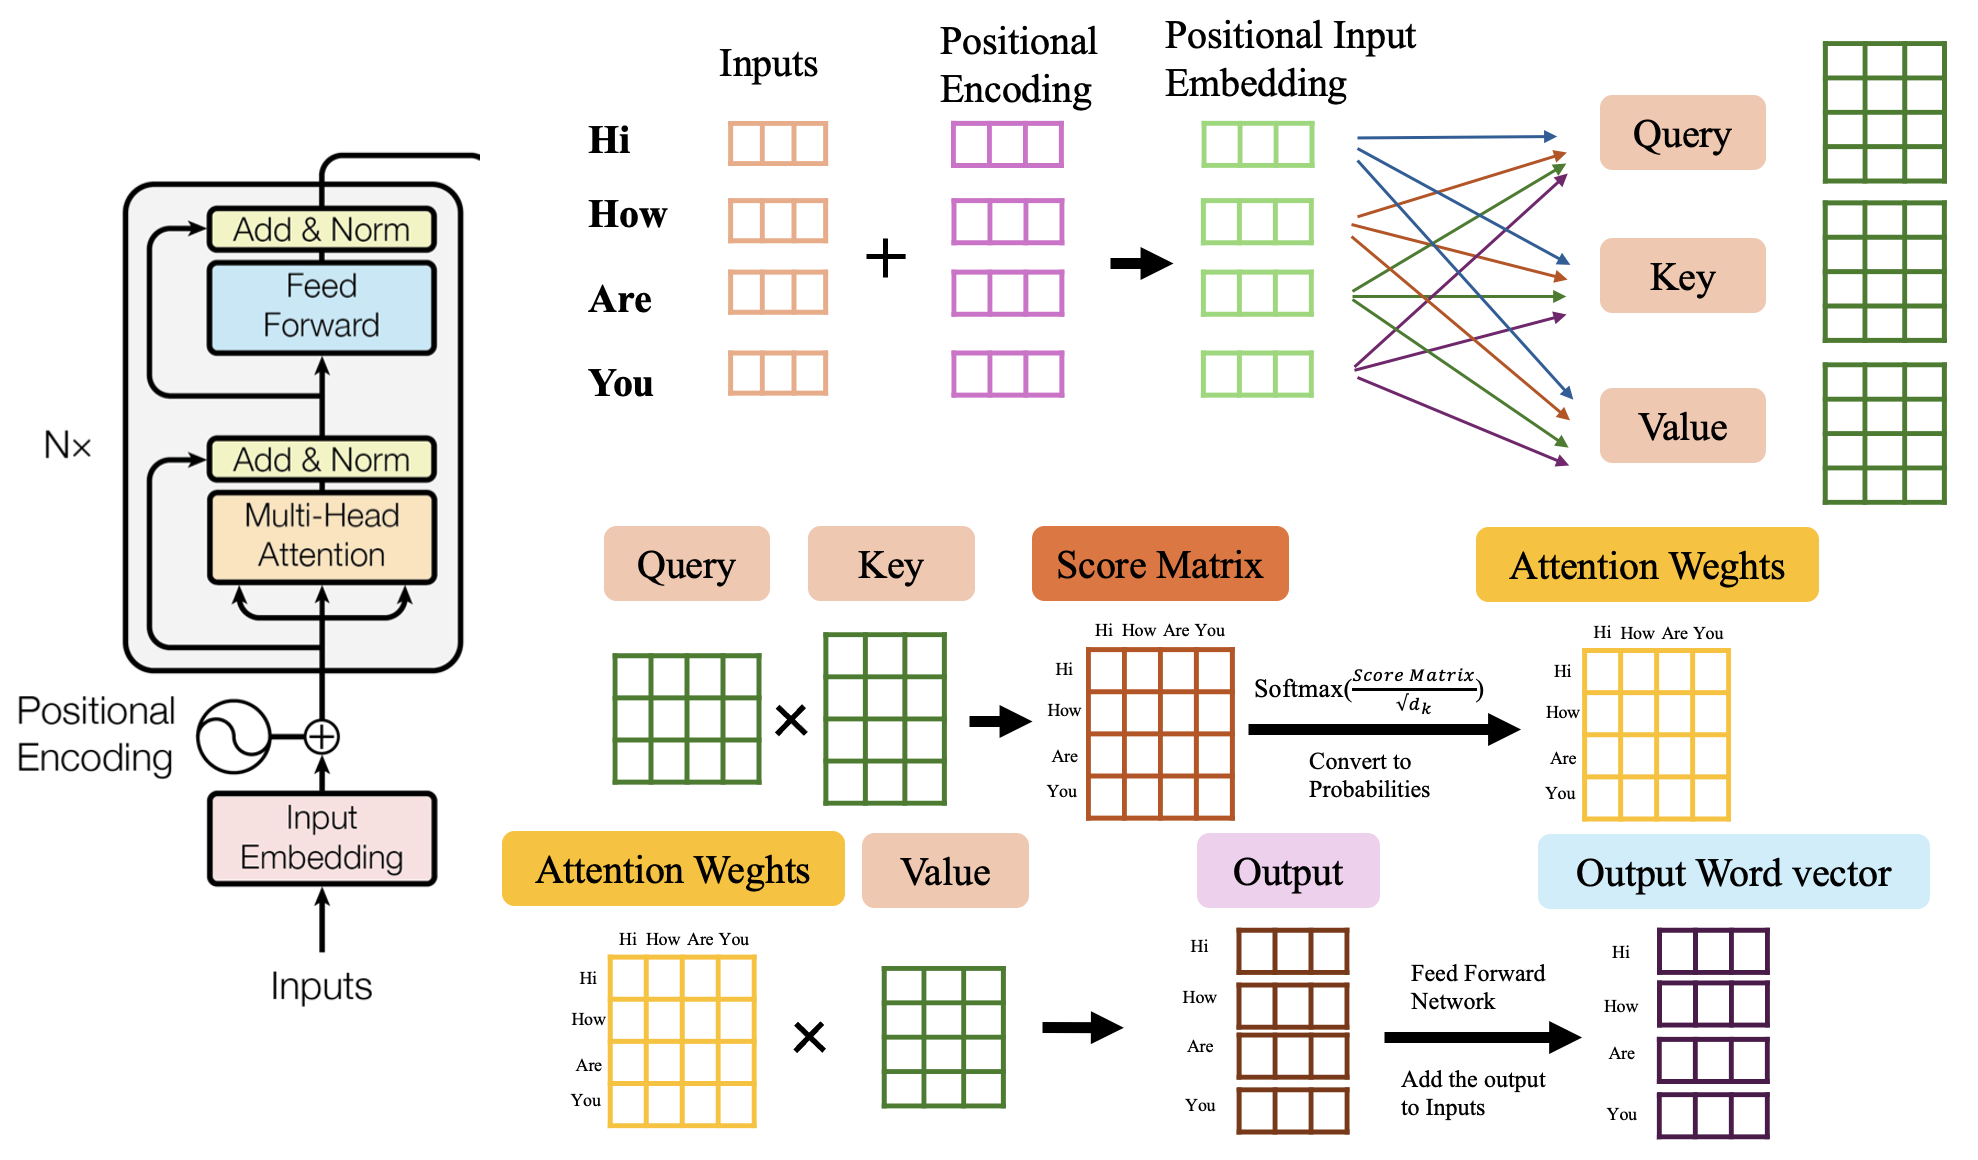
\includegraphics[width=0.8\textwidth]{Chapter2/Chapter2Figs/encoder.png}
    \caption{Transformer Encoder}\label{fig: ch0: transformer_encoder}
\end{figure}


\begin{figure}[h]
    \centering
    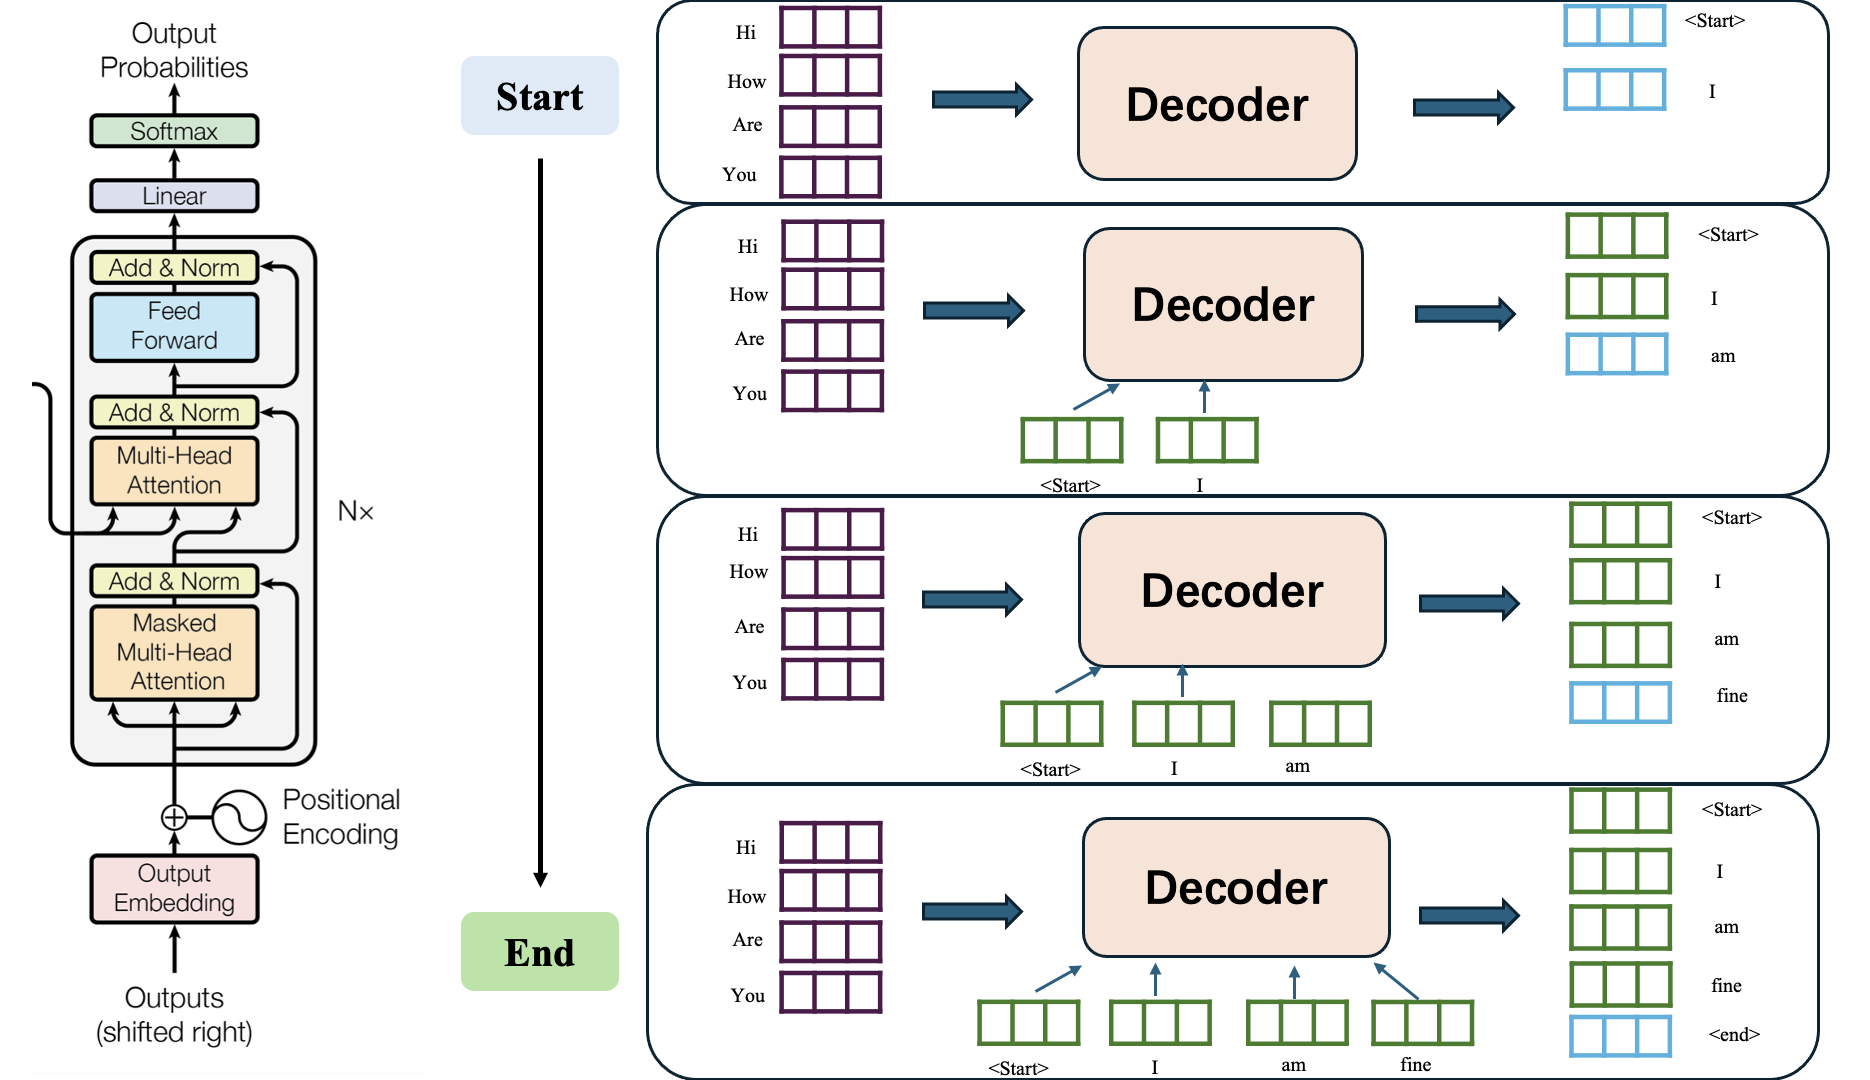
\includegraphics[width=0.8\textwidth]{Chapter2/Chapter2Figs/decoder.png}
    \caption{Transformer Decoder}\label{fig: ch0: transformer_decoder}
\end{figure}


There are two well known implementations of transformer are the Generative Pre-trained Transformer (GPT, \cite{gpt2018}) and the Bidirectional Encoder Representations from Transformer (BERT, \cite{bert2018}). The GPT which based on the Decoders of the transformer and pre-trained word vectors is used for generating text, such as the ChatGPT. On the other hand, the BERT is based on the Encoder of the transformer, used for understanding text, like the Google search. Moveover, the reduced computational cost makes a deeper and larger neural network available in text generation. For instance, the GPT-3 has 175 billion parameters and 96 layers (\cite{brown2020language}). The complexity and depth of the network allows the model to capture more features in the texts, which can be used to generate human-like outputs. 




\subsection{Consistent Texts}\label{ch2:sec:lr:text}
The development of LLMs has significantly advanced the field of Natural Language Processing (NLP), enabling the generation of high-quality, human-like text. However, the models, like GPT and BERT, are pre-trained on a various range of datasets. Ensuring the consistency of generated text remains a challenge. Consistency refers to the logical coherence and factual accuracy of the text across different sections or throughout a document. 

% TODO: add some thing about COT 20241226

% Chain-of-Thought (CoT) prompting is a technique used to improve the reasoning capabilities of language models by breaking down complex tasks into smaller, manageable steps. This method involves guiding the model through a series of intermediate steps, which helps in generating more coherent and logically consistent outputs. CoT prompting can be particularly useful in tasks that require multi-step reasoning, such as mathematical problem-solving, logical reasoning, and generating structured documents like FOMC Minutes. By incorporating CoT prompting, we can enhance the model's ability to produce high-quality, contextually relevant text that aligns with the desired output format.


% LLMs, such as GPT and BERT, are pre-trained on vast datasets and can generate text that is contextually relevant and grammatically correct. However, these models sometimes produce text that lacks consistency, especially when generating longer documents or when the context changes significantly within the text.



Meanwhile, sometime, the pre-trained data may not be suitable for the user. Because the model is trained on a wide range of general public texts. But, users can re-train the model with their own dataset using a technique so called fine-tuning, even if the dataset size is small. There are two kinds of methods for fine-tuning, full parameter and partial parameter (see Fig. \ref{fig: ch0: transformer_finetuning}). Full parameter fine-tuning will update parameters in all the layers inside the model, while partial parameter fine-tuning will frozen part of the layers and only update particular layers or add extra layers. Fine-tuning can improve the performance of the model on a specific task. For instance, the Llama model, which serves as the base model for text generation, has been fine-tuned into two distinct models: Llama Chat, optimized for conversational purposes, and Llama Code, which is specialized for coding tasks (\cite{llama-recips}). Therefore, our research will utilize the remarkable generating ability of the LLM. We will try to fine-tune a LLM with our own dataset, aim to provide a consistent synthetic structured texts using the model.


\begin{figure}[h]
    \centering
    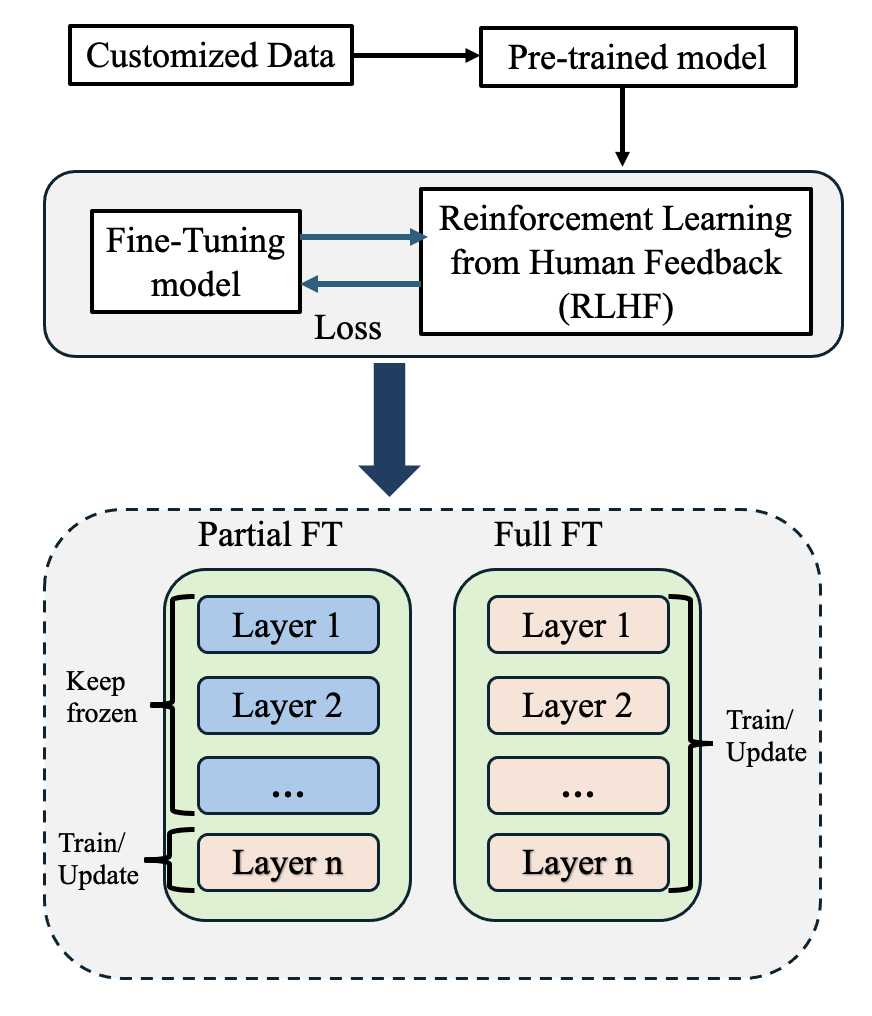
\includegraphics[width=0.3\textwidth]{Chapter2/Chapter2Figs/finetuning.png}
    \caption{Transformer Fine-Tuning}\label{fig: ch0: transformer_finetuning}
\end{figure}




\section{The Dataset}\label{ch2:sec:the dataset}
% Theseminutes were written from a third-person perspective and often included many specific details,attributing specific policy views to individual FOMC members

The FOMC meetings have been recorded since the committee's formation under the Banking Act of 1935 (\cite{todd2016corollary}). Initially, from 1936 to 1967, the minutes were released only once a year in these early years. Between 1967 and 1992, the minutes were named as ``the Minutes of Actions''. combined with ``the Record of Policy Actions'', these documents provided detailed insights not only into the policies but also the reasoning and proceedings behind them. Starting in 1993, a timely record of all policy issues and decisions made by the Committee was published after each meeting, although the documentation lacked a structured format. After 2009, the minutes were organized into distinct sections, including "Economic Situation," "Financial Situation," "Economic Outlook," and "Committee Policy Action," and the Committee has continued to use this structure to the present day. Therefore, we have chosen to use the minutes post-2009 as our primary source material.



First of all, we downloaded the data from Jan 2009 to May 2024 from the Federal Reserve System Website. For FOMC Minutes, there are 119 documents in total. We first separate the entire Minutes into sub-sections, ``Staff Review of the Economic Situation'', ``Staff Review of the Financial Situation'', ``Staff Economic Outlook'', ``Participants' Views on Current Conditions and Economic Outlook'', and ``Committee Policy Actions''. There are 486 sections in total. Although some other sections may be included in the Minutes, for instance, there is a ``Developments in Financial Markets and the Federal Reserve`s Balance Sheet'' in the 20090624 Minutes, these five sections are all included in the Minutes after 2009. We also downloaded the Minutes before 2009 (1963-2009), but these documents do not contain all these five parts. Hence these documents are used as supplementary training materials. 

On average, each Minutes contains 15,119 tokens. There are 1,401,485 tokens in the dataset. Tokens are integer numbers representing different ``words'', which serve as inputs for the model. 

Notably, the term ``word'' in this context does not strictly refer to whole words. Instead, LLMs operate on ``sub-words'' or ``tokens'', which are components of words. For instance, ``Negative'' might be tokenized as ``Neg'' and ``agtive'' to reduce the size of the dictionary, which is known as token dictionary or tokenizer. Each LLM has its unique tokenizer. More powerful LLMs typically have larger tokenizers. For instance, ChatGPT-4's tokenizer contains 256,000 tokens, while LLAMA3's tokenizer includes 128,000 tokens. Table \ref{tab:ch2:summary_statis} provides the summary statistics for the tokens.

% Notably, LLM utilize sub-words rather than entire words. Sub-words are segments of words, such as ``tive'', ``sion'', and ``ing'', which help increase the model's efficiency. The transaction from a ``word'' to some ``tokens'' is facilitated by the tokenizer, which functions similarly to a dictionary of tokens and sub-words. Generally, a more powerful model will have a larger tokenizer. For instance, the LLAMA2's tokenizer has 8K entries, while LLAMA3's contains 128K. 

\begin{table}[h]
    \scriptsize
    \centering
    \begin{tabular}{p{3.8cm}cccccccc}
        \toprule
        Names&                                                Count&	    Mean&	    Std&	 Min&	   25\%&	  50\%&	   75\%&	Max \\
        \hline
        Total Minutes&	                                        123&	15119.50&	5136.89&	8144&	  10545&	 13117&	  20234&	25106 \\
        Total Sections&	                                        486&	 2883.71&	2921.00&	 294&	 1391.5&	1729.5&	3014.75&	13621\\
        Staff Economic Outlook&	                                123&	 3002.20&	 779.20&	 294&	   2556&	  3076&	   3481&	5080 \\
        Staff Review of the Economic Situation&	                120&	 1348.81&	 314.13&	 653&	1178.25&	  1356&	   1490&	2929 \\
        Staff Review of the Financial Situation&	            119&	 1491.61&	 291.48&	 903&	   1293&	  1479&	 1643.5&	2461 \\
        Committee Policy Action&	                            122&	 5625.28&	4646.81&	1262&	   1770&	2448.5&	  11118&	13621 \\
        Staff Review of the Economic and Financial Situation&	  2&	    3286&	 200.82&	3144&	   3215&	  3286&	   3357&	3428 \\
        \bottomrule
    \end{tabular}
    \caption{Summary Statistics for Tokens of Different Sections and Minutes}
    \label{tab:ch2:summary_statis}
\end{table}


As the maximum length for the major sections are less than 4096 tokens (except the ``Committee Policy Action''), we conduct a cutoff on the text and set the maximum length of the ``Assistant Prompt'' as 4096 to reduce the memory usage. 


Furthermore, the dataset size may not be big enough to conduct fine-tuning. Therefore, we downloaded extra texts as supplementary training materials, including the Transcripts, Green books, Blue books, for re-pre-train the model. The FOMC Transcripts for the corresponding Minutes are the detailed record of the meetings. The FOMC Green books (from 1990 to 2010) contain the detailed analysis of the economic and financial data, and the Blue books (from 1990 to 2010) demonstrate the corresponding economic and financial backgrounds. Table \ref{tab:ch2:summary_supplementary_materials} lists the summary statistics for our supplementary materials.


\begin{sidewaystable}[htp]
    \centering
    \footnotesize
    \begin{tabular}{c c c c c p{10cm}}
        \toprule
        Name&	Start Year&	End Year&	Count&	Average Tokens& \hspace{3.2cm} Description \\
        \hline
        Blue Book&	1965&	2010&	424&	15175.19&  The Blue Book, entitled ``Monetary Policy Alternatives'' includes the background and the context on the alternative monetary policy that the committee could consider.\\
        Green Book&	1964&	2010&	140&	33753.46&  The Green Book, named ``Current Economic and Financial Conditions'', provides in-depth analysis of the U.S. and international economy. \\
        Beige Book&	2010&	2019&	15&	    21298.2& The Beige Book, entitled ``Summary of Commentary on Current Economic Conditions by Federal Reserve District'', provides information on current economic from different district.\\
        Teal Book A&	2010&	2024&	69&	71786.20& The Teal Book A, officially subtitled ``Economic and Financial Conditions: Current Situation and Outlook'', provides in-depth analysis and forecasts of the U.S. and international economy (Same as Green Book) and analysis of financial market developments\\
        Teal Book B&	2010&	2024&	69&	24426.38& The Teal Book B, officially subtitled ``Monetary Policy: Strategies and Alternatives'', provide background and context on monetary policy alternatives that the FOMC could consider at a particular meeting.(Same as Blue Book)\\
        \makecell[c]{Summary of Economic Projection\\ (SEP)}&	2007&	2019&	20&	7385.30&  The SEP includes a compilation and summary of these projections (which includes individual projections without attribution) is circulated to participants, and a detailed summary of the economic projections\\
        \bottomrule
    \end{tabular}
    \caption{Summary of Supplementary Materials} 
    \label{tab:ch2:summary_supplementary_materials}
\end{sidewaystable}

% The Bluebook, officially entitled "Monetary Policy Alternatives," was produced by the staff of the Board of Governors to provide background and context on monetary policy alternatives that the FOMC could consider
% The Greenbook, officially entitled "Current Economic and Financial Conditions," provided in-depth analysis of the U.S. and international economy.
% The Beige Book, known as such originally for its beige cover, is officially entitled "Summary of Commentary on Current Economic Conditions by Federal Reserve District."
% collects anecdotal information on current economic conditions in its District

% Tealbook A, officially subtitled “Economic and Financial Conditions: Current Situation and Outlook,” produced by the staff of the Board of Governors, provides in-depth analysis and forecasts of the U.S. and international economy that were previously covered by Parts 1 and 2 of the Greenbook, and also provides analysis of financial market developments that was previously covered in the Bluebook.
% Tealbook B, officially subtitled “Monetary Policy: Strategies and Alternatives,” is produced by the staff of the Board of Governors to provide background and context on monetary policy alternatives that the FOMC could consider at a particular meeting. Tealbook B includes the same information that had been included in the Bluebook, except that the financial developments content was moved to Tealbook A.
% submit individual economic projections in conjunction with four FOMC meetings a year. A compilation and summary of these projections (which includes individual projections without attribution) is circulated to participants, and a detailed summary of the economic projections




% Bluebook: The Bluebook, officially entitled "Monetary Policy Alternatives," was produced by the staff of the Board of Governors to provide background and context on monetary policy alternatives that the FOMC could consider at an upcoming meeting from 1965 to 2010. It was distributed to FOMC participants during the week before an FOMC meeting--usually one day after the Greenbook.

% Greenbook: The Greenbook, officially entitled "Current Economic and Financial Conditions," provided in-depth analysis of the U.S. and international economy. It was produced by the staff at the Board of Governors and  distributed to FOMC meeting attendees the week before the meeting from 1964 to 2010. For most of its history, the Greenbook was split into two parts plus a supplement:

% Part 1: Current Economic and Financial Conditions: Summary and Outlook
% Part 2: Current Economic and Financial Conditions: Recent Developments
% Supplement: Current Economic and Financial Conditions: Supplemental Information



% Tealbook: Bluebook and Greenbook were merged in June 2010

% Statement on Longer-Run Goals and Monetary Policy Strategy: First released in January 2012, this statement articulates the framework for monetary policy and serves as the foundation for the Committee's policy actions.


% Beige Books: The Beige Book, known as such originally for its beige cover, is officially entitled "Summary of Commentary on Current Economic Conditions by Federal Reserve District." It is produced by Reserve Bank staff and released to the public approximately two weeks prior to each regularly scheduled FOMC meeting.




Then, we extracted the numerical data to assemble our input prompts from WRDS (Financial Data) and FRED Economic Data (Macroeconomic Data). For economic analysis, we extracted the U.S. Macro Data including monthly CPIs, monthly Federal Fund Rates, quarterly GDPs, and monthly Unemployment Rates. For financial data, we downloaded the monthly S\&P 500 Index level and the monthly U.S. Treasury Note yields (2-Year, 5-Year, and 10-Year), Then, we calculated the return for these data:

\begin{equation*}
    R_{i, t} = \frac{Y_{i, t} - Y_{i, t-1}}{Y_{i, t-1}} \times 100
\end{equation*}

where $i$ is the corresponding data, including CPI, Federal Fund Rate, GDP, Unemployment Rate, S\&P 500 Index Level, and 10-year US Treasury Rate, $Y_{i, t-1}$ is the data level for the previous time. $Y_{i, t}$ is the current data level.

\section{The Base Model}\label{ch2:sec:llm}
To generate consistent texts using the LLM, we choose to use \textbf{LLAMA3-8B-Instruct}, the most powerful open-sourced LLM developed by MetaAI (\cite{meta2024llama3}), as our base model. The LLAMA family is released with three main sizes, ``LLAMA-8B'', ``LLAMA-70B'', and ``LLAMA-405B''. LLAMA3-8B is the smallest model in LLAMA3 family but can be deployed on a single GPU with 24 GB of memory. \textbf{LLAMA3-8B-Instruct} is further fine-tuned on human-like conversations optimized for dialogue and chat. Noticeably, the maximum context length supported by the model is 128,000 tokens, which is suitable for a FOMC minutes. 


% modifications
Notably, compared with the traditional transformer architecture (\cite{vaswani-etal2018}), the model has incorporated modifications to enhance training stability and generation quality. 

% grouped-query attention (GQA)

First of all, the model adopted Grouped-Query Attention (GQA, \cite{ainslie2023gqa}) in place of Multi-Query Attention (MQA, \cite{vaswani-etal2018}) and Multi-Head Attention (MHA, \cite{vaswani-etal2018}). While MHA can produce high-quality outputs, it demands significant memory capacity. Conversely, MQA significantly reduces memory usage but at the cost of lower generation quality. However, GQA can generate outputs comparable to MHA with similar memory requirements to MQA, making it suitable for processing long contexts.

% SwiGLU
Additionally, the Swish Gated Linear Unit (SwiGLU, Eq. \eqref{eq:ch2:swiglu}, \cite{shazeer2020glu}) replaces the Rectified Linear Unit (ReLU, Eq. \eqref{eq:ch2:relu}, \cite{glorot2011deep}) in the activation function. Extra gate layers are introduced in the model to enhance performance, particularly in managing long contexts.


\begin{equation}\label{eq:ch2:relu}
    ReLU (\mathbf {x} )=\max(0,\mathbf {x} '\mathbf{W} + \mathbf{b})
\end{equation}


\begin{equation}\label{eq:ch2:swiglu}
    \begin{split}
        Swish_{\beta}(\mathbf{y}) &= \mathbf{y} \cdot sigmoid(\mathbf{y}' \mathbf{\beta}) = \frac{\mathbf{y}}{1 + exp(-\mathbf{y}' \mathbf{\beta})} \\
        SwiGLU(\mathbf{x}, \mathbf{W_1}, \mathbf{W_2}, \mathbf{b}, \mathbf{c}) &= Swish_{1}(\mathbf{x}' \mathbf{W_1} + \mathbf{b}) \otimes (\mathbf{x}' \mathbf{W_2} + \mathbf{c})
    \end{split}
\end{equation}

where $\mathbf{x} \in \mathbb{R}^{n \times m}$ is the output from previous layer, $\mathbf{W_1} \in \mathbb{R}^{k \times m \times n}$, $\mathbf{W_2} \in \mathbb{R}^{k \times m \times n}$, $\mathbf{b} \in \mathbb{R}^{n}$, and $\mathbf{c} \in \mathbb{R}^{n}$ are trainable parameters, with $\mathbf{W_1}$ and $\mathbf{W_2}$ are weights, $\mathbf{b}$ and $\mathbf{c}$ are bias terms. $\mathbf{W_2}$ and $\mathbf{c}$ serve as parameters for the gate layer.


% \cite{su2024roformer}
% rotary positional embeddings (RoPE)
Finally, the model incorporates Rotary Positional Embeddings (RoPE, \cite{su2024roformer}), which encodes both the absolute and relative position information of tokens using a rotation matrix, unlike the original transformer that employed a sinusoidal function to encode only absolute position.

Overall, the modifications, including the Grouped-Query Attention (GQA) and the Swish Gated Linear Unit (SwiGLU), alongside the Rotary Positional Embeddings (RoPE), constitute significant advancements in the model. These enhancements not only optimize the model's performance but also broaden its applicability across a diverse range of complex NLP tasks. Consequently, these improvements position LLAMA as a comparable model among leading large language models (LLMs).




\section{Model Training}

To enhance the model's capability in economic and financial analysis, we employed Supervised Fine-Tuning (SFT) and Group Relative Policy Optimization (GRPO) for Reinforcement Learning (RL). Firstly, SFT utilizes a high-quality question-answer (Q\&A) dataset to train the model to directly produce outputs that closely align with the target answers. Subsequently, to further optimize the analytical capabilities of the model, we implemented Reinforcement Learning (RL), guiding the model to refine its policy based on provided objectives.


\subsection{Model Input}
To start with, we reformat our dataset into the specific templates for our SFT and GRPO. 

For SFT, each input consists of three parts (denoted as $input^{SFT}_i = (q_i, o^{SFT}_i)$, $o^{SFT}_i = (c_i, a_i)$): Question ($q_i$), Reasoning ($c_i$), and Answer ($a_i$). Firstly, the reasoning process and the finally answer will be combined as the model's target output. Then, the input will be reformatted into a Q\&A pair. During the SFT, the model will generate a output ($o_i^* = (c^*_i, a^*_i)$) based on the given question ($q_i$). The target of SFT to minimize the loss ($\mathcal{L}^{SFT}$) between the $(c^*_i, a^*_i)$ and $(c_i, a_i)$.


For RL training, we only use Questions ($input^{RL}_i = q_i$) as our input. The model will generate the output ($o^{RL}_i = (c_i, a_i)$) by optimizing a given reward function ($\mathcal{R}$)


\subsection{Supervised Fine-Tuning}
In this section, we explain the input for the Supervised Fine-Tuning (SFT). The SFT process aims at enhancing model's ability in financial analysis. The model will learn to generate a logical reasoning process and draw a similar conclusion as the required output. For example, we want to conduct an analysis on the current inflation rate. We use Personal Consumption Expenditures (PCE) Index as the key indicator. We construct the input prompt ($q_i$) as (Table \ref{tab:ch2:sft_user_prompt_example}):

\begin{table}[h]
    \centering
    \footnotesize
    \begin{tabular}{p{0.98\textwidth}}
    \toprule
    \textbf{User Prompt ($q_i$):} \\
    \midrule
    You are an economist preparing briefing notes for the Federal Open Market Committee (FOMC) meeting on \textbf{2023-07-26 00:00:00}. Your task is to analyze recent trends in \textbf{Personal Consumption Expenditures (PCE)} and related indicators, writing in the tone and style of the \textbf{Developments in Financial Markets and Open Market Operations} section of the FOMC minutes. \\
    
    Use neutral, data-driven, and measured language throughout your response. \\
    
    Your analysis \textbf{must} be based on the following indicators: 
    \begin{itemize}
        \item \texttt{Personal Consumption Expenditures Index (Index 2017=100, Seasonally Adjusted).csv}
        \item \texttt{Personal consumption expenditures by major function (Index numbers, 2017=100; quarters and months are seasonally adjusted).xlsx}
        \item \texttt{Personal consumption expenditures by major function (Millions of dollars; quarters and months are seasonally adjusted at annual rates).xlsx}
    \end{itemize}

    Using the accompanying data tables from the past two years provided below: \\

    \vspace{0.5em}
    \textbf{Indicators: Personal Consumption Expenditures (PCE)} \\
    \texttt{Personal Consumption Expenditures Index (Index 2017=100, Seasonally Adjusted).csv} \\
    
    \begin{tabular}{|l|l|}
    \hline
    \texttt{observation\_date} & \texttt{PCEPI} \\
    \hline
    2021-08-01 & 109.72 \\
    2021-09-01 & 110.047 \\
    \vdots & \vdots \\
    2023-06-01 & 120.435 \\
    2023-07-01 & 120.598 \\
    \hline
    \end{tabular} \\

    \vspace{0.5em}
    Keep your response focused, analytically rigorous, and under 4096 tokens. \\
    \bottomrule
    \end{tabular}
    \caption{SFT User Prompt Example}
    \label{tab:ch2:sft_user_prompt_example}
\end{table}



The target output consists of the Reasoning process ($c_i$) and Answer ($a_i$), we firstly wrapped the Reasoning process using \textbf{\texttt{\textless think\textgreater ... \textless /think\textgreater}} and the Answer using \textbf{\texttt{\textless answer\textgreater ... \textless /answer\textgreater}}. Then we combined these two parts as our target output ($o_i = (c_i, a_i)$)(Table. \ref{tab:ch2:sft_target_output_example}):

\begin{table}[h]
    \centering
    \footnotesize
    \begin{tabular}{p{0.98\textwidth}}
    \toprule
    \textbf{Target Output ($o_i = (c_i, a_i)$):} \\
    \midrule
    \textbf{\textless think\textgreater} Okay, I need to prepare a briefing note for the FOMC meeting based on the provided data. The user wants an analysis of recent trends in PCE and related indicators, structured like the \textquotedblleft Developments in Financial Markets and Open Market Operations\textquotedblright{} section from the FOMC minutes. The tone needs to be neutral, data-driven, and measured. Let's start by looking at the data given. \\

    First, the Personal Consumption Expenditures Index (PCEPI) shows a steady increase from 109.72 in August 2021 to 120.598 in July 2023. The monthly growth rates have slowed in recent months. \\

    ... ... \\

    Finally, tie this into the broader economic context, like the potential for a delayed recession and inflation moving towards 2\% by 2025 as per the survey mentioned in the example. \\

    Make sure the language is neutral, avoid speculation, and stick strictly to the data provided. Use terms like ``moderated'', ``deceleration'', ``partially offset'', and ``notable contributions''. Structure the analysis into sections: overall PCE trends, sectoral breakdown, and implications for inflation outlook. Avoid mentioning any data not provided, and ensure all points are backed by the numbers given. \textbf{\textless /think\textgreater} \\[1ex]

    \textbf{\textless answer\textgreater} \textbf{Developments in Personal Consumption Expenditures and Implications for Inflation} \\

    Recent data through July 2023 indicate sustained growth in personal consumption expenditures (PCE), albeit with moderating momentum in key categories. The PCE Price Index (PCEPI) rose to 120.60 in July 2023, reflecting a 3.6\% year-over-year increase, down from the 5.9\% pace observed in July 2022. Monthly gains have decelerated notably, with the index advancing at an average rate of 0.16\% over the three months ending in July. \\

    ... ... \\

    While consumption growth remains positive, real outlays are being constrained by tighter financial conditions and moderating excess savings. This dynamic supports a baseline of below-trend GDP growth with incremental labor market rebalancing, reducing the risk of entrenched inflation expectations. However, the resilience in wage-sensitive services categories warrants continued vigilance regarding price-setting behavior. \textbf{\textless /answer\textgreater} \\
    \bottomrule
    \end{tabular}
    \caption{SFT Target Output Example}
    \label{tab:ch2:sft_target_output_example}
\end{table}


The refinement of the model through retraining employs stochastic gradient descent (SGD) to iteratively adjust the model parameters ($\theta$) based on the \textit{loss function}. In partial fine-tuning (Partial FT), the update process selectively modifies certain layers while leaving others unchanged by zeroing out their gradients. This targeted approach enables the model to adapt to new tasks while preserving the knowledge learned during pre-training.

During Supervised-Fine-tuning (Supervised-FT), the \textit{loss} is calculated as the discrepancy between the model's generated responses ($\bm{o^*} \in R^{m\times n}$) and the target responses ($\bm{o}^{SFT} \in R^{m \times n}$). This discrepancy is quantified by the multi-class Cross Entropy Loss ($\mathcal{L}^{CE}$):


\begin{equation*}
  \mathcal{L}^{CE} = -\frac{1}{n}\sum_{i=1}^{n} o^{SFT}_{k, i}\log  o^*_i(y_i|x_1, x_2, \dots,x_m, y_1, y_2, \dots, y_{i-1}; \theta)
\end{equation*}



where $o_{k,i} = [o_1, o_2, \cdots, o_k, \cdots, o_m]$ is a unit vector with $o_k = 1$ (also known as one-hot encoded vector), which represents the target token, $o^*_i(\cdot)$ denotes the probabilities for the predicted token given the input tokens $\bm{x}$ and previously generated words $\bm{y}$, which are always smaller than 1. Here, the $n$ is the total number of words in the generated response sequence. The Cross Entropy Loss ($\mathcal{L}_{CE}$) represents sum of the negative log probabilities that the model assigns to the target tokens. The correct probabilities will occur when $o_{k,i}=o^*_i(\cdot) = 1$ and $\mathcal{L}^{CE}=0$. Therefore, the objective of the SFT is to minimize $\mathcal{L}^{CE}$ by updating the model's weights $\theta$.  






\subsection{Reinforcement Learning}
% Reinforcement Learning (RL) requires the model to update the parameters ($\theta$) by optimizing the feedback. Here, we employed Group Relative Policy Optimization (GRPO) in this stage.

Reinforcement Learning (RL) requires the model to update parameters ($\theta$) by optimizing feedback. Different from the Supervised Fine-Tuning, the target of the Reinforcement Learning is to maximize the feedback by changing the way of producing the output. As the same analysis can be constructed in different ways, RL serves as a significantly in booting the model's reasoning ability, such as the ChatGPT o1 (\cite{jaech2024openai}) and the Deepseek-R1 (\cite{guo2025deepseek}) for general purpose, the Fin-R1 \cite{liu2025fin} and the Fino1 \cite{qian2025fino1} in finance domain.

More specifically, in this stage, we employed Group Relative Policy Optimization (GRPO, \cite{shao2024deepseekmath}).

GRPO is an on-policy reinforcement learning algorithm derived from the Proximal Policy Optimization algorithm (PPO, \cite{schulman2017proximal}). PPO is a policy-gradient-based reinforcement learning technique designed for stable optimization. It requires the model to maximize a reward signal ($A_t$), provided by a reward function, by generating outputs from the current policy model ($\pi_{\theta}$). Unlike Supervised Fine-Tuning, RL does not rely on predefined target outputs. Instead, it uses a scoring function to evaluate model outputs. This score, known as the reward, serves as feedback for model training. The goal of training is to maximize an objective function ($\mathcal{J}(\theta)$) defined in terms of the reward. Consequently, only the question ($q_i$) is included in the training input ($input^{RL}_i$).


Additionally, PPO employs a clipping function ($CLIP(\cdot)$) to scale the reward in the objective function, enhancing training stability. The model parameters ($\theta$) are updated using stochastic gradient descent (SGD) until the objective function is maximized. The objective function ($\mathcal{J}^{\text{PPO}}$) is given by:




\begin{footnotesize}
    \begin{equation}
        \begin{split}
            \mathcal{J}^{\text{PPO}}(\theta) =
             &\mathbb{E}_{q\sim P(Q), o\sim\pi_{\theta_{\text{old}}}(O|q)}\frac{1}{|o|}\sum_{t=1}^{|o|}\Bigg[\min\Bigg\{ \\
             &\frac{\pi_{\theta}(o_t | q, o_{<t})}{\pi_{\theta_{\text{old}}}(o_t | q, o_{<t})} A_t(r_t, v_t), \text{CLIP}\left(\frac{\pi_{\theta}(o_t | q, o_{<t})}{\pi_{\theta_{\text{old}}}(o_t | q, o_{<t})}, 1 - \epsilon, 1+\epsilon\right)A_t(r_t, v_t)\Bigg\}\Bigg]
        \end{split}
    \end{equation}
\end{footnotesize}



where:

\begin{equation*}
r_t = r_\phi(q, o_{\leq t}) - \beta \log\frac{\pi_{\theta}(o_t | q, o_{<t})}{\pi_{\text{ref}}(o_t | q, o_{<t})}
\end{equation*}

\begin{equation*}
v_t = V_t(o_t | q, o_{<t})
\end{equation*}

Here, $\pi_{\theta}$ represents our trainable \textit{policy model}. $r_t$ is the KL-divergence adjusted reward, where $r_\phi$ is the reward from the \textit{reward model}. $\pi_{\text{ref}}$ is the \textit{reference model}, initialized as a copy of the original policy model. $V_t(\cdot)$ denotes a trainable \textit{value model} used to estimate expected rewards, aiding the policy in exceeding baseline expectations. $A_t$ is the advantage function, providing final feedback to the model, typically calculated using Generalized Advantage Estimation (GAE). $\beta$ is the penalty coefficient for KL divergence, while $\epsilon$ controls the extent of clipping. Both $\beta$ and $\epsilon$ are hyperparameters crucial for maintaining training stability.

However, the training cost for the PPO is significantly higher than the Supervised Fine-Tuning. In PPO, four models, the policy model, the reference model, the reward model, and the value model, need to be loaded. Two models, the policy model and the value model, are being trained at the same time. To address the issue, we employed the Group Relative Policy Optimization (GRPO), which removed the value model by calculating the relative average reward from multiple sampled outputs as the advantage. The objective function for GRPO ($\mathcal{J}^{\text{GRPO}}$) is given by:




\begin{footnotesize}
    \begin{equation}
        \begin{split}
            \mathcal{J}^{\text{GRPO}}(\theta) 
            &= \mathbb{E}_{q \sim P(Q), \{o\}^G_{i=1} \sim \pi_{\theta_{\text{old}}}(O \mid q)} \Bigg[ \frac{1}{G} \sum_{i=1}^{G} \frac{1}{|o_i|} \sum_{t=1}^{|o_i|} \Bigg\{ \nonumber \\
            &\quad \min \Bigg( 
                \frac{ \pi_{\theta}(o_{i,t} \mid q, o_{i,<t}) }{ \pi_{\theta_{\text{old}}}(o_{i,t} \mid q, o_{i,<t}) } \hat{A}_{i,t}(r_{i,t}), \;
                \text{CLIP}\left( \frac{ \pi_{\theta}(o_{i,t} \mid q, o_{i,<t}) }{ \pi_{\theta_{\text{old}}}(o_{i,t} \mid q, o_{i,<t}) }, 1 - \epsilon, 1 + \epsilon \right) \hat{A}_{i,t}(r_{i,t}) 
            \Bigg) \nonumber \\
            &\quad - \beta \, \mathbb{D}_{\text{KL}}\left[ \pi_{\theta} \,\|\, \pi_{\text{ref}} \right] 
            \Bigg\} \Bigg]
        \end{split}
    \end{equation}
\end{footnotesize}




where:

\begin{equation*}
    \hat{A}_{i,t}(r_{i, t}) = \frac{r_{i, t} - \text{mean}(\mathbf{r}_t)}{\text{std}(\mathbf{r}_t)}
\end{equation*}

\begin{equation*}
    \mathbb{D}_{KL}[\pi_{\theta} || \pi_{ref}] = \frac{\pi_{\text{ref}}(o_{i, t} | q, o_{i, <t})}{\pi_{\theta}(o_{i, t} | q, o_{i, <t})} - \log \frac{\pi_{\text{ref}}(o_{i, t} | q, o_{i, <t})}{\pi_{\theta}(o_{i, t} | q, o_{i, <t})} - 1
\end{equation*}


Here, $G$ is the size of the sampled outputs for each iteration $t$. $r_{i,t}$ is reward for output $i$ at iteration $t$. Instead of training a \textit{value model} in calculating the expected rewards, the GRPO uses the sum of the normalized rewards from a sample outputs of size $G$ as the advantage function $\hat{A}_{i,t}$. Additionally, the KL divergence penalty is added directly to the objective function to reduce the calculation cost in the advantage function. As a result, the training cost has been significantly reduced by applying the GRPO. 

Finally, to implement the GRPO, we use the same \textit{User Prompt ($q_i$)} (see Table \ref{tab:ch2:sft_user_prompt_example}) as the SFT stage as our input. Then, we adopt the idea of ``LLM as Judge'' by using another powerful model as our reward model to score the output from our policy model.



\subsection{Reward Function Design}
Inspired from the literature, we adopt a two aspect reward function, format reward and accuracy reward. However, different from mathematical reasoning, there is no ``correct answer'' in economic and financial analysis. Therefore, we use another LLM evaluating the reasoning process and the final analysis. We purpose several key points are the criteria in evaluation. The model will mark the output and return a score as the reward.

\subsubsection{Format Reward}
To ensure the reasoning process, we require the model to generate the output in the specific format. The reasoning process should be wrapped with \textbf{\texttt{\textless think\textgreater ... \textless /think\textgreater}} and the answer should be wrapped with \textbf{\texttt{\textless answer\textgreater ... \textless /answer\textgreater}}. Therefore, we designed a format reward function ($\mathcal{R}_{fmt}(\cdot)$) checking the output. A correct format will be scored as 1 while the wrong format will be marked as 0:


\begin{equation*}
    \mathcal{R}_{\text{fmt}}(o_i) = 
    \begin{cases}
        1, & \text{if the format is correct} \\
        0, & \text{if the format is wrong}
    \end{cases}
\end{equation*}




\subsubsection{Accuracy Reward}

Unlike previous studies that trained their models on publicly available datasets, such as FinQA (\cite{chen2021finqa}), our training target is to generate comprehensive and logical economic and financial analyses. Since there is no fixed or predefined correct answer for such analyses, we adopt the "LLM as Judge" framework (\cite{zheng2023judging}) for our reward model. Instead of creating a mathematical reward function, we design a prompt that includes the model's generated output. Then, we employ a powerful evaluation model (referred to as the \textit{"reward model"}, denoted by $\mathcal{R}_{acc}(\cdot)$) to score the output based on specific instructions. The resulting score serves as the accuracy reward. However, the reward obtained through this method heavily depends on the quality and clarity of the instructions provided; biased evaluation criteria may lead to biased rewards. To mitigate this issue, we carefully designed seven evaluation dimensions: problem definition, data usage, theoretical support, empirical analysis, analytical depth, policy relevance, and language accuracy. Table \ref{tab:ch2:llm_as_judge_evaluation} summarizes these seven aspects along with a brief description of each criterion. 




\begin{table}[h]
    \centering
    \footnotesize
    \begin{tabular}{p{0.33\textwidth}|p{0.63\textwidth}}
    \toprule
    \textbf{Evaluation Dimension} & \textbf{Evaluation Focus} \\
    \midrule
    \textbf{1. Problem Definition \& Structural Completeness} &
    \parbox[t]{0.65\textwidth}{
        \textbullet\ Is the core research or policy question clearly defined? \newline
        \textbullet\ Is there sufficient background and objective? \newline
        \textbullet\ Is the structure complete (e.g., introduction, method, findings, conclusion)?\newline
        \textbullet\ Is the logical flow coherent from question to conclusion?\newline
} \\
\hline
\textbf{2. Data Usage \& Verifiability} &
\parbox[t]{0.65\textwidth}{
    \textbullet\ Are the data selected from credible sources?\newline
    \textbullet\ Are the data sources clearly cited?\newline
    \textbullet\ Are the data relevant to the argument?\newline
    \textbullet\ Can the analysis be independently verified using the data?\newline
} \\
\hline
\textbf{3. Theoretical Support \& Citations} &
\parbox[t]{0.65\textwidth}{
    \textbullet\ Are appropriate economic or financial theories applied?\newline
    \textbullet\ Are relevant scholarly or institutional sources cited?\newline
    \textbullet\ Are the cited theories or sources correctly interpreted?\newline
} \\
\hline
\textbf{4. Empirical Methodology \& Transparency} &
\parbox[t]{0.65\textwidth}{
    \textbullet\ Are the empirical methods appropriate for the question?\newline
    \textbullet\ Are the methods clearly explained and reproducible?\newline
    \textbullet\ Are assumptions and limitations discussed?\newline
} \\
\hline
\textbf{5. Analytical Depth \& Insight} &
\parbox[t]{0.65\textwidth}{
    \textbullet\ Are key variables correctly identified and analyzed?\newline
    \textbullet\ Does the analysis show meaningful economic or financial insight?\newline
    \textbullet\ Are policy trade-offs or complex relationships discussed?\newline
    \textbullet\ Is there a forward-looking or scenario-based component?\newline
} \\
\hline
\textbf{6. Policy Relevance \& Real-world Significance} &
\parbox[t]{0.65\textwidth}{
    \textbullet\ Are the conclusions tied to real-world policy implications?\newline
    \textbullet\ Does the analysis provide decision-relevant insights?\newline
    \textbullet\ Is the analysis useful for policymakers or market actors?\newline
} \\
\hline
\textbf{7. Clarity \& Language Accuracy} &
\parbox[t]{0.65\textwidth}{
    \textbullet\ Is the language clear, professional, and grammatically correct?\newline
    \textbullet\ Are economic and financial terms used accurately?\newline
    \textbullet\ Is the terminology consistent throughout the analysis?\newline
} \\
\bottomrule
    \end{tabular}
    \caption{Evaluation Criteria for Assessing LLM-Generated Economic/Financial Analyses}
    \label{tab:ch2:llm_as_judge_evaluation}
\end{table}




% ## TODO: add the details about each point



Finally, each criterion is scored on a scale from 1 to 5, where 1 indicates "Very Poor" and 5 represents "Excellent." The total score obtained by summing these individual criterion scores is then used as the accuracy reward. We utilize the following prompt to encapsulate our policy model's output before submitting it to the reward model:




\begin{table}[h]
    \centering
    \footnotesize
    \begin{tabular}{p{0.98\textwidth}}
    \toprule
    \textbf{Prompt for Accuracy Reward ($\mathcal{R}_{\text{acc}}(o_i)$):} \\
    \midrule
    You are an economic and financial policy expert serving as an internal evaluator at the Federal Reserve. You are tasked with \textbf{assessing the analytical quality and fidelity} of a large language model's output based on structured economic/financial data. \\[1ex]

\textbf{Evaluation Criteria (Score each from 1--5):} \\

-- Problem Definition \& Structural Completeness \\
\quad \textit{... description ...} \\

-- Accuracy of Economic Relationships and Logic \\
\quad \textit{... description ...} \\

-- Correct Use of Data and Trends \\
\quad \textit{... description ...} \\[1ex]

\textbf{Scoring Instructions:} \\
- Each category receives an integer score (1--5). \\
-  Justify each score briefly and concisely. \\[1ex]

\textbf{Output Template:} \\
- \textbf{Score}: \texttt{\textbackslash boxed\{\{X\}\}} \\
- \textbf{Justification}: Your explanation in 1--2 sentences. \\[1ex]

\textbf{Input Data:} \\
The model analysis is based on the following indicators: \texttt{\{emphasized\_label\}}. \\

\textbf{\textless Provided Data\textgreater} \\
\texttt{\{provided\_data\}} \\
\textbf{\textless /Provided Data\textgreater} \\[1ex]

\textbf{\textless Model Analysis\textgreater} \\
\texttt{\{model\_analysis\}} \\
\textbf{\textless /Model Analysis\textgreater} \\
\bottomrule
    \end{tabular}
    \caption{Accuracy Reward Prompt}
    \label{tab:ch2:accuracy_reward_prompt}
\end{table}




\section{Consistent Text Generation}\label{ch2:sec:text generation}

In this section, we will attempt to generate the FOMC Minutes using a Large Language Model (LLM). Fine-tuning large pre-trained models is a highly effective method for adapting general-purpose LLMs to specific content tasks. This technique enables the model to conform to a particular style, affecting not only the output format but also the semantics. Furthermore, we will employ various approaches to evaluate the performance of the fine-tuned model in this specific task.



\subsection{Pre-Training}\label{ch2:sec:pre_training}

Although Supervised Fine-Tuning (SFT) is a powerful technique for instructing models to generate structured and formatted outputs, it has been criticized for its inability to introduce new knowledge into the model (\cite{gekhman2024does}, \cite{huang2025survey}). Recent studies have confirmed that while SFT can significantly enhance a model's controllability in adapting to specific styles and domains, it does not contribute to knowledge acquisition (\cite{zhang2023instruction}). Almost all of knowledge absorbed by the model occurs during the pre-training phase (\cite{zhou2023lima}).

Meanwhile, continuous pre-training has been shown to be an effective method for incorporating new knowledge into a model (\cite{parmar2024reuse}, \cite{gekhman2024does}). Furthermore, as LLMs are typically pre-trained on a broad range of publicly available texts, they lack domain-specific experience in specialized fields. Given that our task focuses on financial studies rather than general tasks, we employ supplementary materials to further pre-train (re-pretrain) the model, which aims at enhancing its understanding of economic and financial markets.


% ALM, predict next token.

The pre-training stage for LLMs primarily involves two main strategies: the Masked Language Model (MLM) and the Autoregressive Language Model (ALM). In MLM, random words within the text are replaced with a special token such as ``\texttt{[MASK]}'', and the model is trained to predict the masked words based on surrounding context. This approach is particularly effective in improving contextual understanding, especially in encoder-only models such as BERT (\cite{bert2018}). On the other hand, ALM focuses on predicting the next token given a sequence of preceding tokens. This strategy is mainly used by decoder-only models such as ChatGPT (\cite{gpt2018}) and LLaMA (\cite{meta2024llama3}). Therefore, we implement the same strategy in our research. We will mask random token and ask the model to predict the token by minimize the Cross Entropy Loss:

\begin{equation}
    \mathcal{L}_{CE}^{pretrain} = - p(y_{i})\log  q(y_i|y_1, y_2, \dots, y_{i-1}; \theta)
\end{equation}

Where $y_{i}$ is the predicted token. $p(\cdot)$ is the probability distribution of the token, which is 1 if $y_{i}$ is the target token, otherwise it is 0. In this case, $(\cdot) = 1$ as our target token is given. $q(\cdot)$ is the probability of the predicted token by the model, which is always smaller than 1. The $\mathcal{L}_{CE}^{pretrain}$ will be 0 only if $p(y_{i}) = 1$ and $q(\cdot) = 1$. Therefore, the objective for the pre-training is to minimize the $\mathcal{L}_{CE}^{pretrain}$ by updating the parameters $\theta$. 








\subsection{Supervised Fine-tuning}\label{ch2:sec:model finetuning}
After re-pre-training, we will next try to fine-tune the base model (\textbf{LLAMA3B-8-Instruct}). 4 main steps involves in fine-tuning. Firstly, we need to prepare training dataset and convert the FOMC Minutes to the format of input for the model. Then, we need to design system and user prompts. Well-structured prompts can help the model generate logical outputs. After that, we employ quantization method, such as LoRA, for partial-parameter FT to reduce the computational costs. Finally, the the loss will be calculated by comparing the target response with the output generated by the model. The process will keep iterating until the convergence of the loss function. Fig. \ref{fig:ch2:ft_detail} illustrates the fine-tuning process:

\begin{figure}
    \begin{center}
        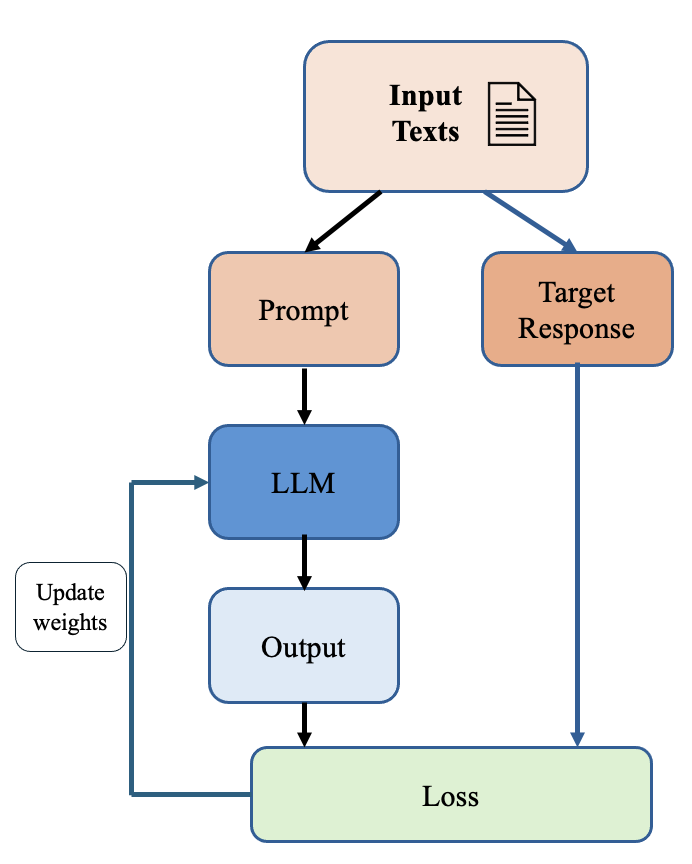
\includegraphics[width=0.3\textwidth]{Chapter2/Chapter2Figs/ft_detail.png}
      \end{center}
      \caption{Fine-Tune Process Flow Chart}
      \label{fig:ch2:ft_detail}
\end{figure}


\subsubsection*{Step 1: Prepare Training Dataset}
Each LLM has its own required format of inputs. All the texts wil be converted to the form of Q\&A pairs. Fig. \ref{fig:ch2:qa_label} shows the labels for LLAMA3, where \textcolor{blue}{$<|$start\_header\_id$|>$} and \textcolor{blue}{$<|$end\_header\_id$|>$ $\setminus$n$\setminus$n} are indicators for the role of the following messages. \textcolor{blue}{$<|$begin\_of\_text$|>$} is the indicator of the start of the conversation. \textcolor{blue}{$<|$eot\_id$|>$} is the indicator of the end of the conversation. An example is provided in  Fig. \ref{fig:ch2:llama3_input_example}.

\begin{figure}[htbp]
\begin{minipage}[c]{0.48\textwidth}
    \begin{center}
    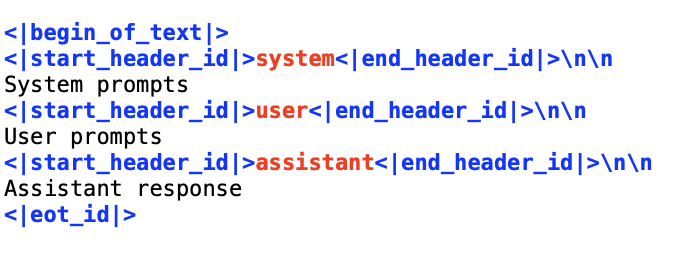
\includegraphics[width=\textwidth]{Chapter2/Chapter2Figs/llama3_template.png}
    \caption{Q\&A Labels for LLAMA3}
    \label{fig:ch2:qa_label}
\end{center}
\end{minipage}
% \hfill
\begin{minipage}[c]{0.48\textwidth}
    \begin{center}
    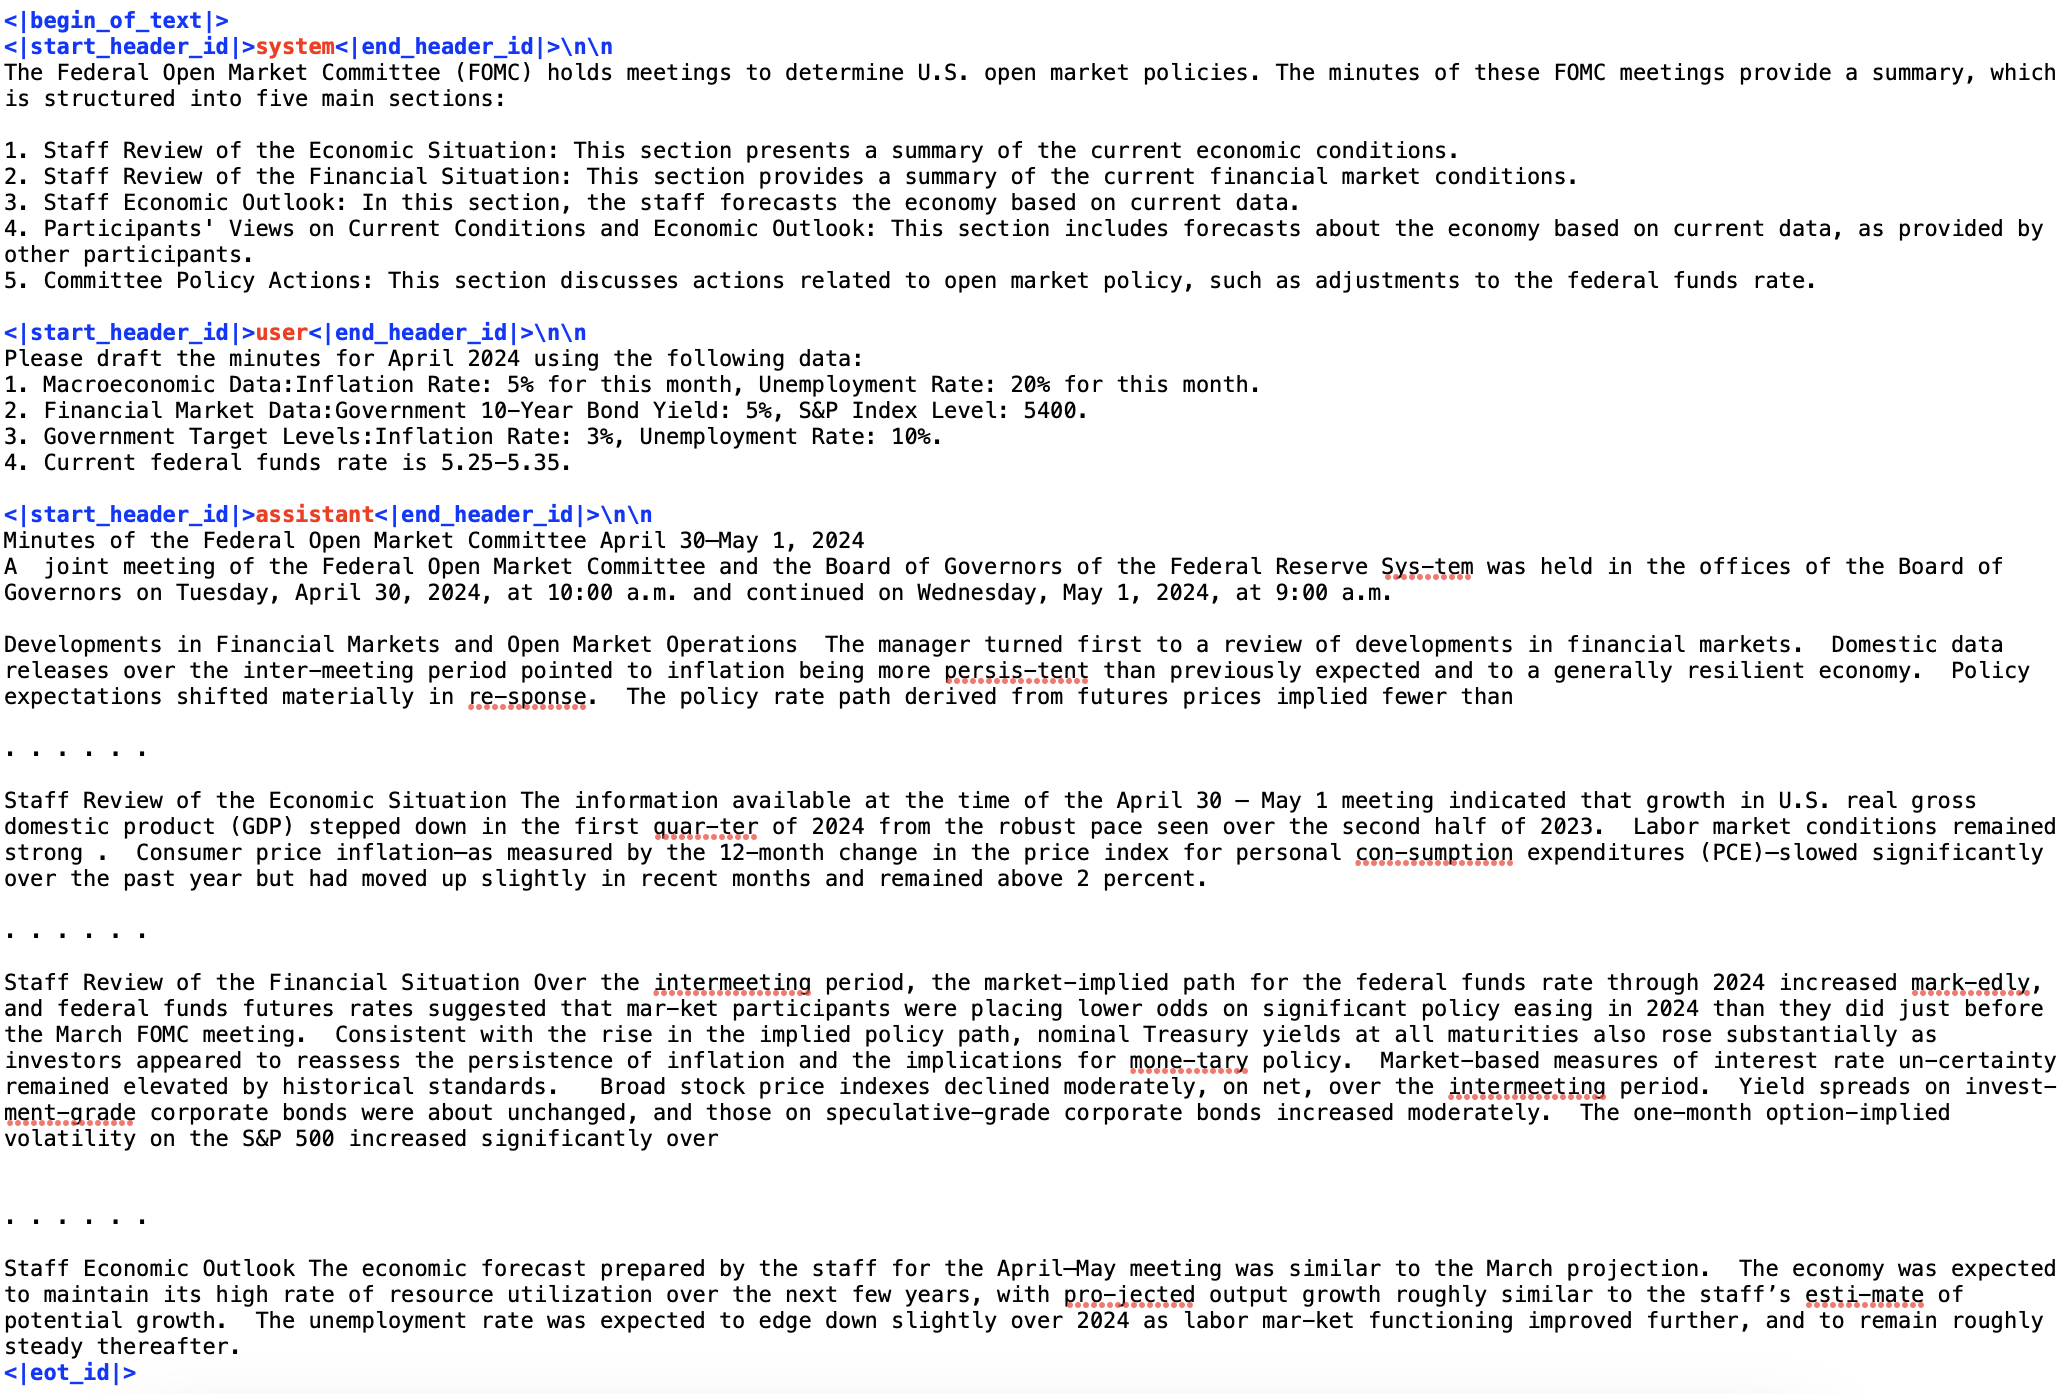
\includegraphics[width=\textwidth]{Chapter2/Chapter2Figs/fomc_example.png}
    \caption{LLAMA3 Input Example}
    \label{fig:ch2:llama3_input_example}
\end{center}
\end{minipage}
\end{figure}
  


\subsubsection*{Step 2: System and User Prompts Engineering}

Prompt engineering plays a pivotal role in eliciting the desired format of text generation from language models. There are three ways in prompting the model, zero-shot standard prompting, zero-shot Chain-of-Though prompting (zero-shot CoT, \cite{kojima2022large}), and few-shot Chain-of-Though prompting (few-shot CoT, \cite{wei2022chain}). 

First of all, the zero-shot standard prompting involves instructing the model to generate the output directly in response to an input prompt. The generated results will be fully replied on the knowledge that the model learned. This approach is effective for straightforward tasks, where the model can do the predict without additional guidance and context. And it shows the model's ability to apply the learned concepts in new scenarios. 

However, for complex reasoning tasks, such as solving mathematical problems or creating an article with interconnected subsections, the Chain of Though (CoT) method yield provide more precise outcomes. 


CoT prompting necessitates the inclusion of guiding instructions within the prompt to aid the model in generating outputs that are more coherent and rational, broken down into manageable steps. There are two ways of CoT, zero-shot CoT and few-shot CoT. Zero-shot CoT is particularly adept at handling mathematical calculations. This method only requires to add an extra sentence in the prompt: ``Answer the question step by step'', which can encourage the model dissect the question into sub-questions. However, for logical reasoning, few-shot CoT outperforms than other methods. Unlike Zero-shot CoT, Few-shot CoT prompting requires a series of interaction between user and the model, dividing the task into several sub-tasks, and addressing each sub-task at each talk. In the context of our research, instead of requiring the model to generate the entire chapters, we adapt a section-by-section approach by asking model to generate a section at each time.  Here we design a four-step process to assist the model in composing complete Minutes. Figure \ref{fig:ch2:cot_steps} illustrates the first three steps in the few-shot CoT. Also, standard prompt steps are listed in Figure \ref{fig:ch2:standard_steps}.

\begin{figure}
    \begin{center}
        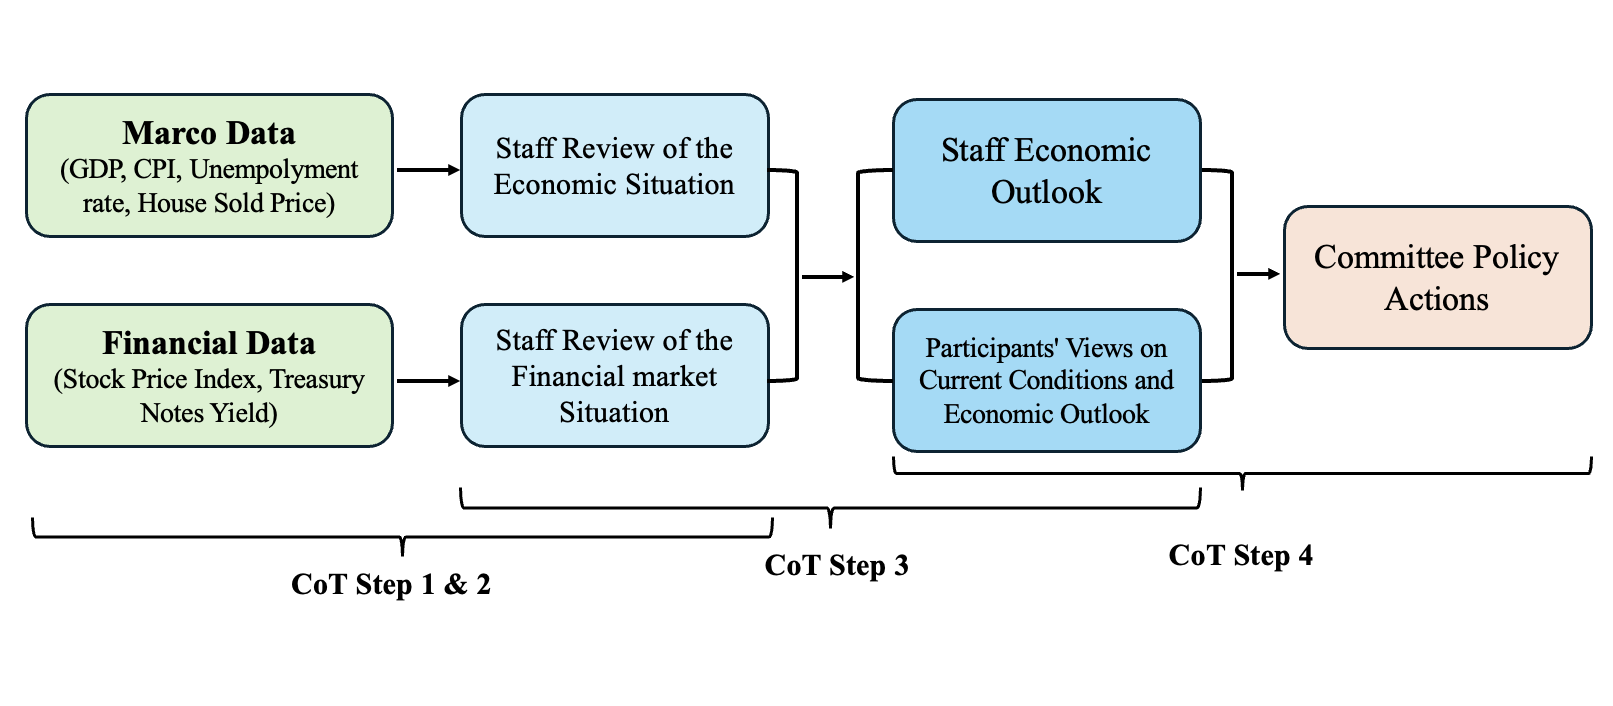
\includegraphics[width=\textwidth]{Chapter2/Chapter2Figs/cot_steps.png}
        \caption{Chain-of-Though Prompt Steps}
        \label{fig:ch2:cot_steps}
    \end{center}
\end{figure}


\begin{figure}
    \begin{center}
        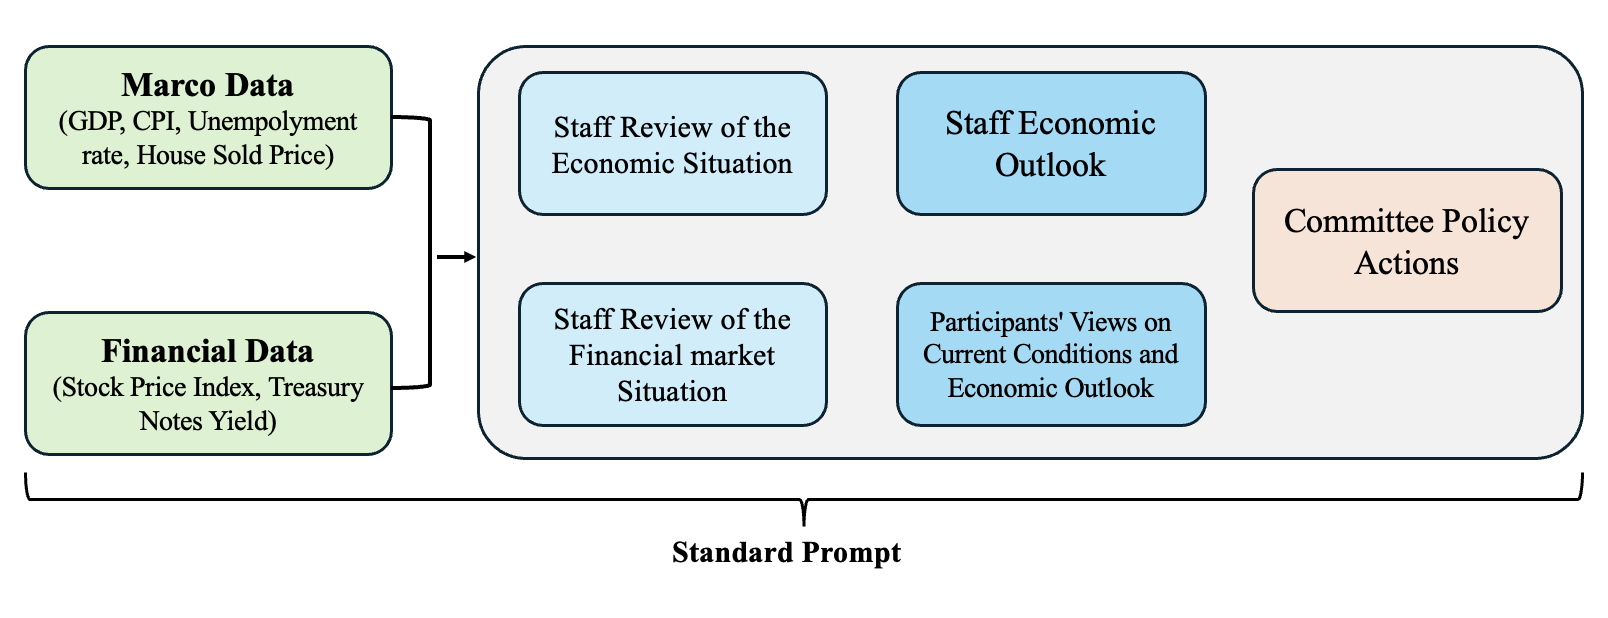
\includegraphics[width=\textwidth]{Chapter2/Chapter2Figs/standard_steps.png}
        \caption{Standard Prompt Steps}
        \label{fig:ch2:standard_steps}
    \end{center}
\end{figure}


Due to constraints on the model's contextual understanding length, our approach involves asking the model to generate a section in the above three steps. Then, in the final step, the model will predict the actions based on the results from the previous steps. Once all sections are developed, they will be combined to form the  complete, synthesized FOMC Minutes.

Table \ref{tab:ch2:cot_prompt} illustrates the prompts in each step in the CoT prompting. In the first step, the model is tasked to generate the ``Staff Review of the Economic Situation'' drawing upon provided macro-economic, and the ``Staff Review of the Financial Situation'' informed by financial data. These two sections are overviews of the current economic and financial conditions based on the statistics. Then, in step 2, the model utilizes these sections to make some prediction about the future scenarios, drafting the ``Staff Economic Outlook'' and the ``Participants Views on Current Conditions and Economic Outlook'', which will affect the Committee's actions on the monetary policy. After that, in step 3, with a comprehensive understanding of the economic and financial contexts, along with predictive insights, the model crafts the "Committee Policy Actions." This section outlines the decisions made regarding monetary policy, informed by the previous summaries and forecasts. Finally, a full synthesized Minutes will be produced by combining all the sections. This iterative process, facilitated through a dialogue-like structure, enables the model to benefit from the cumulative context of previous steps, enhancing the coherence and accuracy of the generated content. 

By structuring the generation process into discrete steps and maintaining a conversational format, we maximize the model's ability to produce high-quality, contextually rich outputs that closely mirror the structure and substance of authentic FOMC Minutes. A detailed example of CoT prompt can be found in Appendix \ref{app:cot_example}. Additionally, we evaluated the performance of using standard prompting to fine-tune the model. Table \ref{tab:ch2:standard_prompt} lists the prompts used in our standard prompting strategy. Notably, a system prompt introducing each section of the Minutes is added as an ``hint'' to the model to maintain the required output format.


\begin{table}[h]
    \centering
    \footnotesize
    \begin{tabular}{p{14cm}}
    \toprule
    \textbf{Step 1: Create connection between ``data'' and ``Review''} \\ 
    \hline
    \textbf{User Prompt:}\\ 
    \hline
    Based on the provided \textcolor{teal}{\{target section name\}} data, please analyze the current economic conditions, using the following guides.\\ 
    $\qquad$ \textcolor{teal}{ \{Instructions\} }
    ~\\
    Here are the \textcolor{teal}{\{target section\}} data from \textcolor{teal}{\{target year start\}} to \textcolor{teal}{\{target minutes data\}}, (all in percentage):\\ $\qquad$ \textcolor{teal}{\{target data name\}}: \textcolor{teal}{\{target data value\}}          \\ 
    \bottomrule
    \toprule
    \textbf{Step 2: Generate ``Outlook'' based on ``Review''} \\ 
    \hline
    \textbf{User Prompt:}\\ 
    \hline
    Based on \textcolor{teal}{\{target section name\}}, predict the future direction of the \textcolor{teal}{\{target section name\}} using the following guide. \\ 
    $\qquad$ \textcolor{teal}{ \{Instructions\}}           \\ 
    \bottomrule
    \toprule
    \textbf{Step 3: Predict ``Action'' based on ``Review'' and ``outlook''} \\ 
    \hline
    \textbf{User Prompt:}\\ 
    \hline
    Create a detailed "Committee Policy Action" section for an FOMC-style meeting record that synthesizes insights from economic and financial market analyses to guide and justify the committee's decisions on monetary policy adjustments.\\
     $\qquad$ \textcolor{teal}{\{Instructions\}}      \\ 
    \bottomrule
    \end{tabular}
    \caption{CoT Prompt Steps}
    \label{tab:ch2:cot_prompt}
\end{table}

\begin{table}[h]
    \centering
    \footnotesize
    \begin{tabular}{p{14cm}}
        \toprule
        \textbf{System Prompt:} \\
        \hline
        The Federal Open Market Committee (FOMC) holds meetings to determine the U.S. open market policies. The minutes of these FOMC meetings provide a summary, which is structured into five main sections: \\
        1. Staff Review of the Economic Situation: This section presents a summary of the current economic conditions.\\
        2. Staff Review of the Financial Situation: This section provides a summary of the current financial market conditions.\\
        3. Staff Economic Outlook: In this section, the staff forecasts the economy based on current data.\\
        4. Participants' Views on Current Conditions and Economic Outlook: This section includes forecasts about the economy based on current data, as provided by other participants.\\
        5. Committee Policy Actions: This section discusses actions related to open market policy, such as adjustments to the federal funds rate. \\
        \hline
        \textbf{User prompts:} \\
        \hline
        Draft the Minutes for \textcolor{teal}{\{date\}} using the following data in the corresponding sections. \\
        $\qquad$ \textcolor{teal}{\{target data name\}}: \textcolor{teal}{\{target data value\}}     \\ 
        \bottomrule
    \end{tabular}
    \caption{Standard Prompt}
    \label{tab:ch2:standard_prompt}
\end{table}





% \paragraph*{Standard Prompt:}
% % #endregion
% \textbf{System prompts}\\
% {\footnotesize
% \textit{``The Federal Open Market Committee (FOMC) holds meetings to determine the U.S. open market policies. The minutes of these FOMC meetings provide a summary, which is structured into five main sections: \\
% 1. Staff Review of the Economic Situation: This section presents a summary of the current economic conditions.\\
% 2. Staff Review of the Financial Situation: This section provides a summary of the current financial market conditions.\\
% 3. Staff Economic Outlook: In this section, the staff forecasts the economy based on current data.\\
% 4. Participants' Views on Current Conditions and Economic Outlook: This section includes forecasts about the economy based on current data, as provided by other participants.\\
% 5. Committee Policy Actions: This section discusses actions related to open market policy, such as adjustments to the federal funds rate.
% ''}}\\
% ~\\
% \textbf{User prompts}\\
% {\footnotesize
% \textit{``Please draft the Minutes for \textcolor{teal}{$<$date$>$} using the following data in the corresponding sections. \\
% 1. Use ``Macroeconomic Data'':  \textcolor{teal}{$<$Macro-economic data$>$} in ``Staff Review of the Economic Situation''\\
% 2. Use ``Financial Market Data'': \textcolor{teal}{$<$Financial Market data$>$} in ``Staff Review of the Financial Situation''\\
% 3. Use ``Government Target Levels'': \textcolor{teal}{$<$Government target level$>$} in All the sections\\
% 4. Use ``Current federal funds rate'' : \textcolor{teal}{$<$Current Federal Fund Rate$>$} in ``Committee Policy Actions''.''}}

% % #endregion
  
\subsubsection*{Step 3: Technique for Partial-Parameter Fine-Tuning}

Fine-tuning (FT) models to enhance their performance on speicific taks is a common practice in the NLP. When conducting Full-parameter Fine-Tuning (FT), the entire base model will be updated, leading to enhanced capabilities in generating task-specific text. However, this comes at a significant computational cost.  Full-parameter fine-tune the model requires about 120GB of GPU memory even only for a 8 billion parameters' model. In contrast, Partial-parameter Fine-Tuning (FT) offers more economical alternative, significantly reducing GPU memory requirements by freezing certain layers of the model.


To further optimize memory usage without compromising on performance, quantization techniques, such as LoRA (Low Rank Adaptation, \cite{hu2021lora}), Quantization Low Rank Adaptation (QLoRA, \cite{dettmers2024qlora}), and Gated Low-Rank Evolving (GaLoRE, \cite{zhao2024galore}), leverage lower precision formats (FP16, FP8, or FP4) to dramatically reduce memory consumption. For instance, LoRA, which has gained prominence for its efficiency in the fine-tuning literature, can decrease memory usage from 120GB to as low as 24GB.

LoRA's mechanism involves introducing additional layers, referred to as Adapters, with a much smaller rank (typically 1 or 2) compared to the pre-trained weight matrices (such as 2048 in the LLaMA3 model). These Adapters are specifically designed for the task at hand and undergo training during the fine-tuning process. Upon completion of training, these adapted layers are merged back into the base model, effectively enhancing its capabilities for the target task while keeping the overall memory footprint minimal. This approach not only facilitates the fine-tuning of large models on resource-constrained environments but also allows for the integration of task-specific knowledge without the need to retrain the entire model from scratch. By strategically updating the parameters in the Adapters, LoRA and similar techniques enable efficient adaptation to new domains or tasks, making them powerful tools in the fine-tuning. For our research , we choose to use QLoRA, a technique combined the traditional LoRA and Quantization, that dramatically increase the fine-tuning efficiency by lower the precision formats to FP4. 



\subsubsection*{Step 4: Minimize the Loss Function}

The refinement of the model through retraining employs stochastic gradient descent (SGD) to iteratively adjust the model parameters based on the \textit{loss function}. In partial fine-tuning (Partial FT), the update process selectively modifies certain layers while leaving others unchanged by zeroing out their gradients. This targeted approach enables the model to adapt to new tasks while preserving the knowledge learned during pre-training.

During Supervised-Fine-tuning (Supervised-FT), the \textit{loss} is calculated as the discrepancy between the model's generated responses ($\bm{Q} \in R^{m\times n}$) and the target responses ($\bm{P} \in R^{m \times n}$). This discrepancy is quantified by the multi-class Cross Entropy Loss ($\mathcal{L}_{CE}$):

\begin{equation*}
  \mathcal{L}_{CE}^{SFT} = -\frac{1}{n}\sum_{i=1}^{n} P_{k,i}\log  Q_i(y_i|x_1, x_2, \dots,x_m, y_1, y_2, \dots, y_{i-1}; \theta)
\end{equation*}

where $P_{k,i} = [p_1, p_2, \cdots, p_k, \cdots,p_m]$ is a unit vector with $p_k = 1$ (also known as one-hot encoded vector), which represents the target token, $Q_i(\cdot)$ denotes the probabilities for the predicted token given the input prompts $\bm(x)$ and previously generated words $\bm{y}$, which are always smaller than 1. Here, the $n$ is the total number of words in the generated response sequence. The Cross Entropy Loss ($\mathcal{L}_{CE}$) represents sum of the negative log probabilities that the model assigns to the target tokens. The correct probabilities will occur when $p_{k,i}=Q_i(\cdot) = 1$ and $\mathcal{L}_{CE}^{SFT}=0$. Therefore, the objective of the SFT is to minimize $\mathcal{L}_{CE}$ by updating the model's weights $\theta$.  



\subsection{Hyperparameter and Training Results}

\subsubsection*{Re-pretraining Results}
For the pretraining stage, we set the learning rate set to 1.0e-4, batch size of 16, and total number of 3 epochs for training. 

% # TODO: add training details on pre-train.

Figure \ref{fig:ch2:pretrain_loss} shows the training loss for our re-pretraining stage.


% learning_rate: 1.0e-4

\begin{figure}
    \begin{center}
        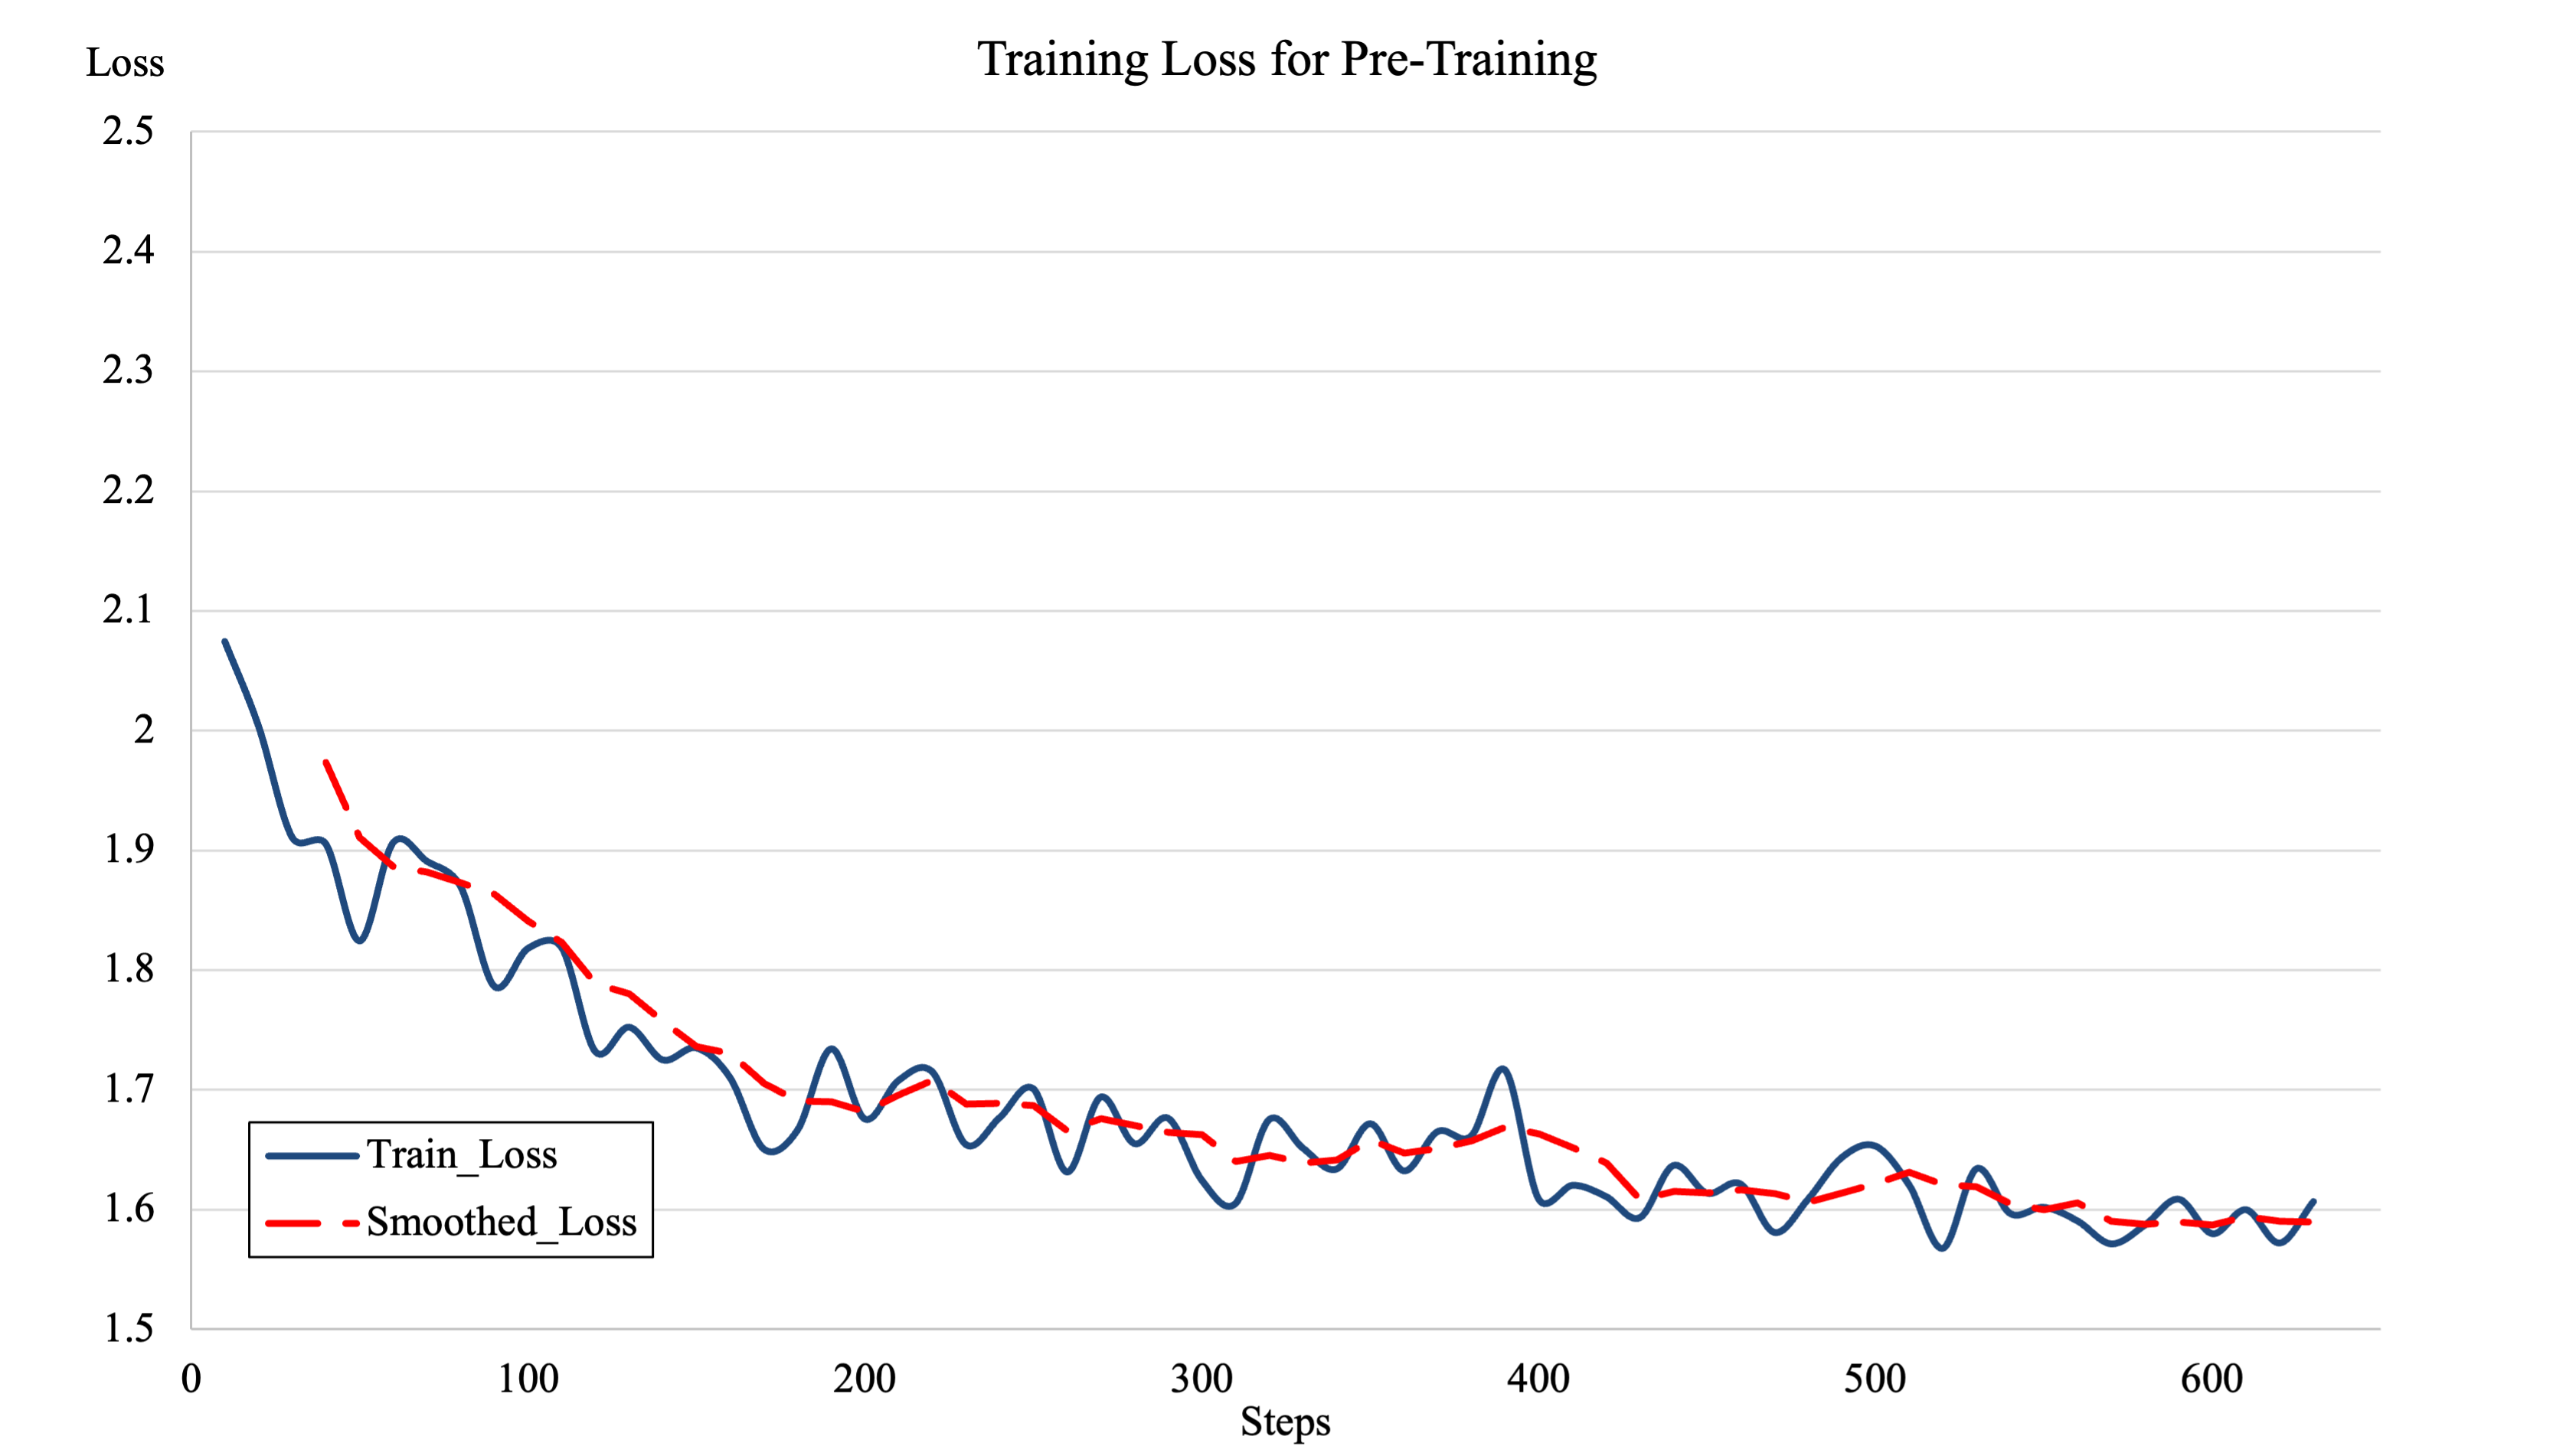
\includegraphics[width=\textwidth]{Chapter2/Chapter2Figs/train_loss_pretrain.png}
      \end{center}
      \caption{Re-Pretraining Loss with 636 Steps}
      \label{fig:ch2:pretrain_loss}
\end{figure}



\subsubsection*{Fine-tuning Results}

The fine-tuning process for the model was configured with a learning rate set to 1.0e-4, batch size of 16, and total number of 9 epochs for training. The temperature parameter was fixed at 0.6, and the top\_p sampling strategy was employed with a value of 0.9. The choice of 16 batch size is due to the limitations of the GPU memory capacity. A higher batch size could significantly reduce training time but would require more memory. Furthermore, given the small sample size and sufficient context length, the entire training dataset was cycled through 9 times (number of epochs = 9) to ensure the a strong link is created between the prompts and the the outputs. Finally, The training loss converge to approximately 0.37 after 243 steps of training with the evaluation loss converging to 0.25.


Initial experiment starts with 10 epochs, as shown in Figure \ref{fig:ch2:training_loss}. During the period, the training loss decreased from 1.6005 (at Step = 10) to 0.2344 (at Step = 270), Simultaneously, the evaluation loss converged from 1.5763 (at Step 10) to 0.3740 after 240 steps and remained stable ending with 0.3678 at step = 270. Notably, while the training loss continued to decline after 270 iterations, the evaluation loss stabilized, indicating the potential onset of overfitting, where the model might become excessively specialized to the training data and lose its generalization capability. Overfitting can significantly degrade a model's utility outside the training environment. Given these observations, we concluded to stop the training at Step 243 and Epoch 9, where both training and evaluation losses were decreasing consistently, showing no significant signs of overfitting.


\begin{figure}[htbp]
    \begin{center}
            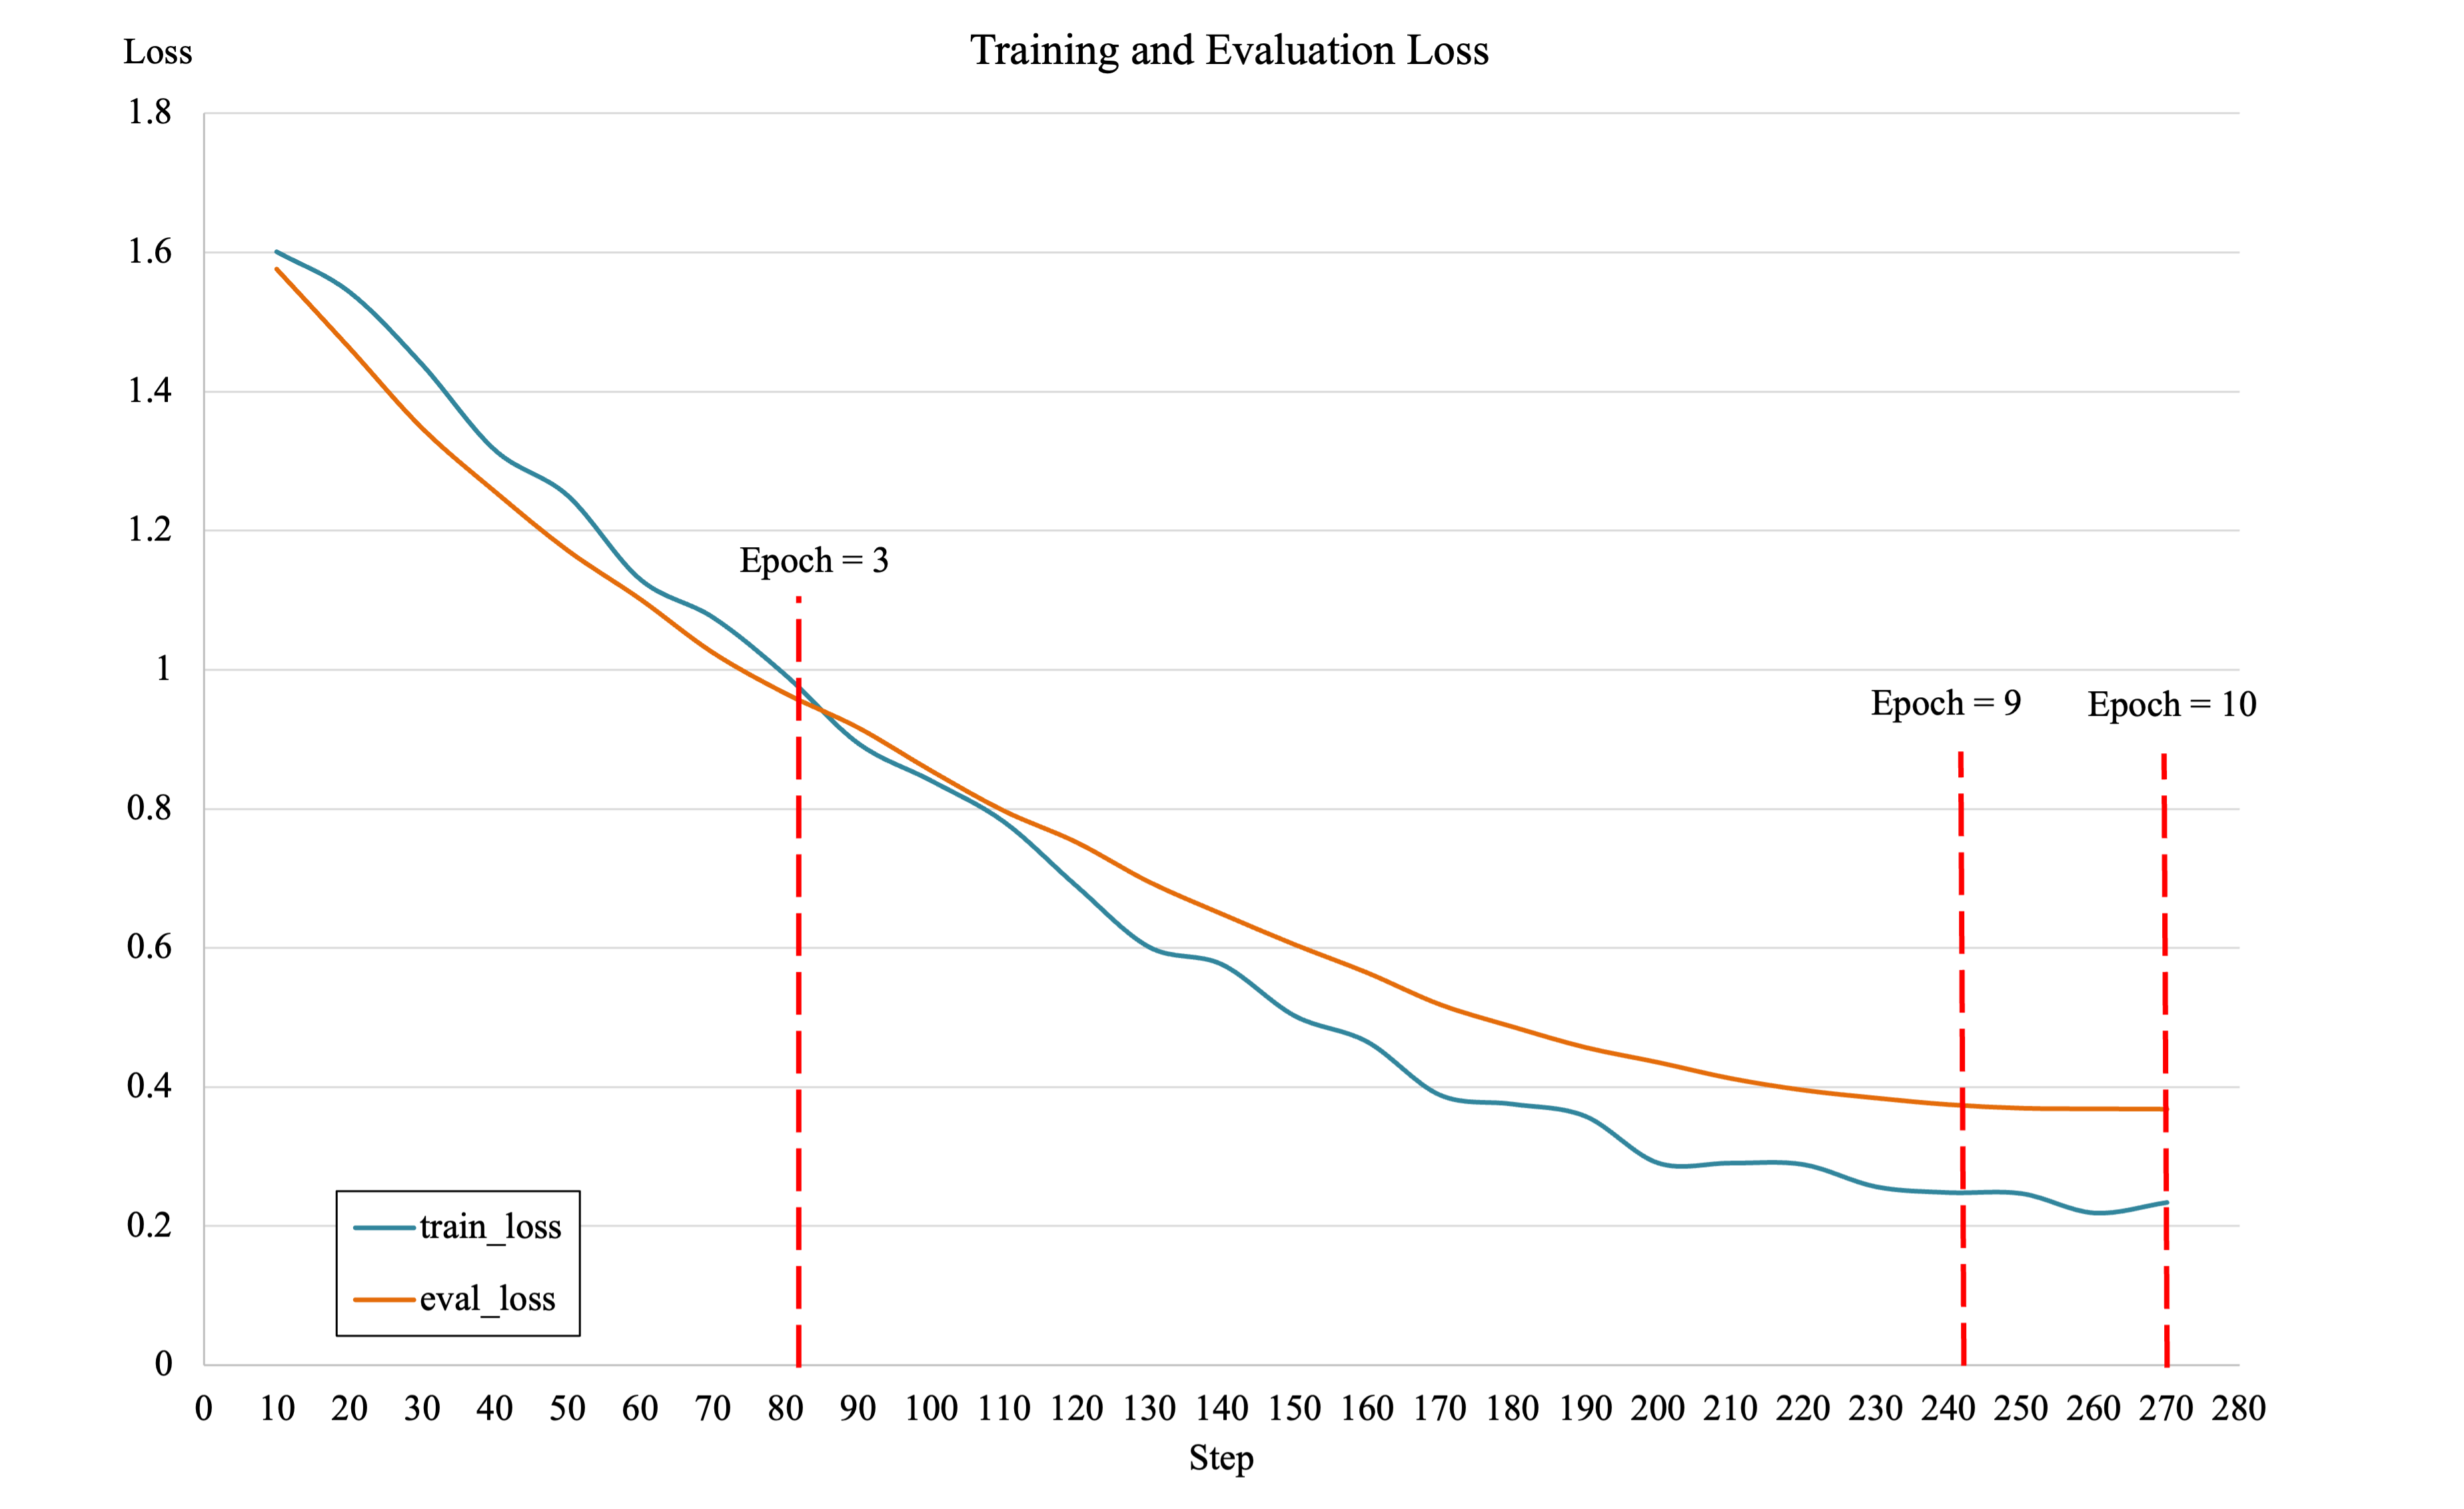
\includegraphics[width=0.9\textwidth]{Chapter2/Chapter2Figs/train_loss_20250111.png}
            \caption{Training Loss and Evaluation Loss}
            \label{fig:ch2:training_loss}
    \end{center}
\end{figure}




Finally, the number of total trainable parameters is 20,971,520 out of 8,051,232,768 total parameters with one adopter (only 0.2605\% trainable rate). We trained the model with 243 steps, each step will use 80\% of the total data (475 sections) as train data, 10\% data (60 sections) for validation.  A separate 10\% portion (60 sections) was designated as the test set prior to initiating the training phase. 



Moreover, we fine-tuned both the base model and the re-pretrain model and compared the fine-tuning training loss for these two models. Figure \ref{fig:ch2:training_loss_compare} illustrates the difference of training and evaluation loss between the base model and the re-pretrained model. Both models converged to a stable loss level after 243 steps, while the re-pretrained model achieved a lower level of both training loss and evaluation loss. The re-pretraining stage has improved a 28.92\% lower in the training loss and 20.10\% in the evaluation loss. The gap is larger with the increasing training epochs. The result is consistent with our expectation and indicates that the re-pretrain process significantly reduce the losses by adding more financial knowledge to the model.  



\begin{figure}[htbp]
    \begin{center}
            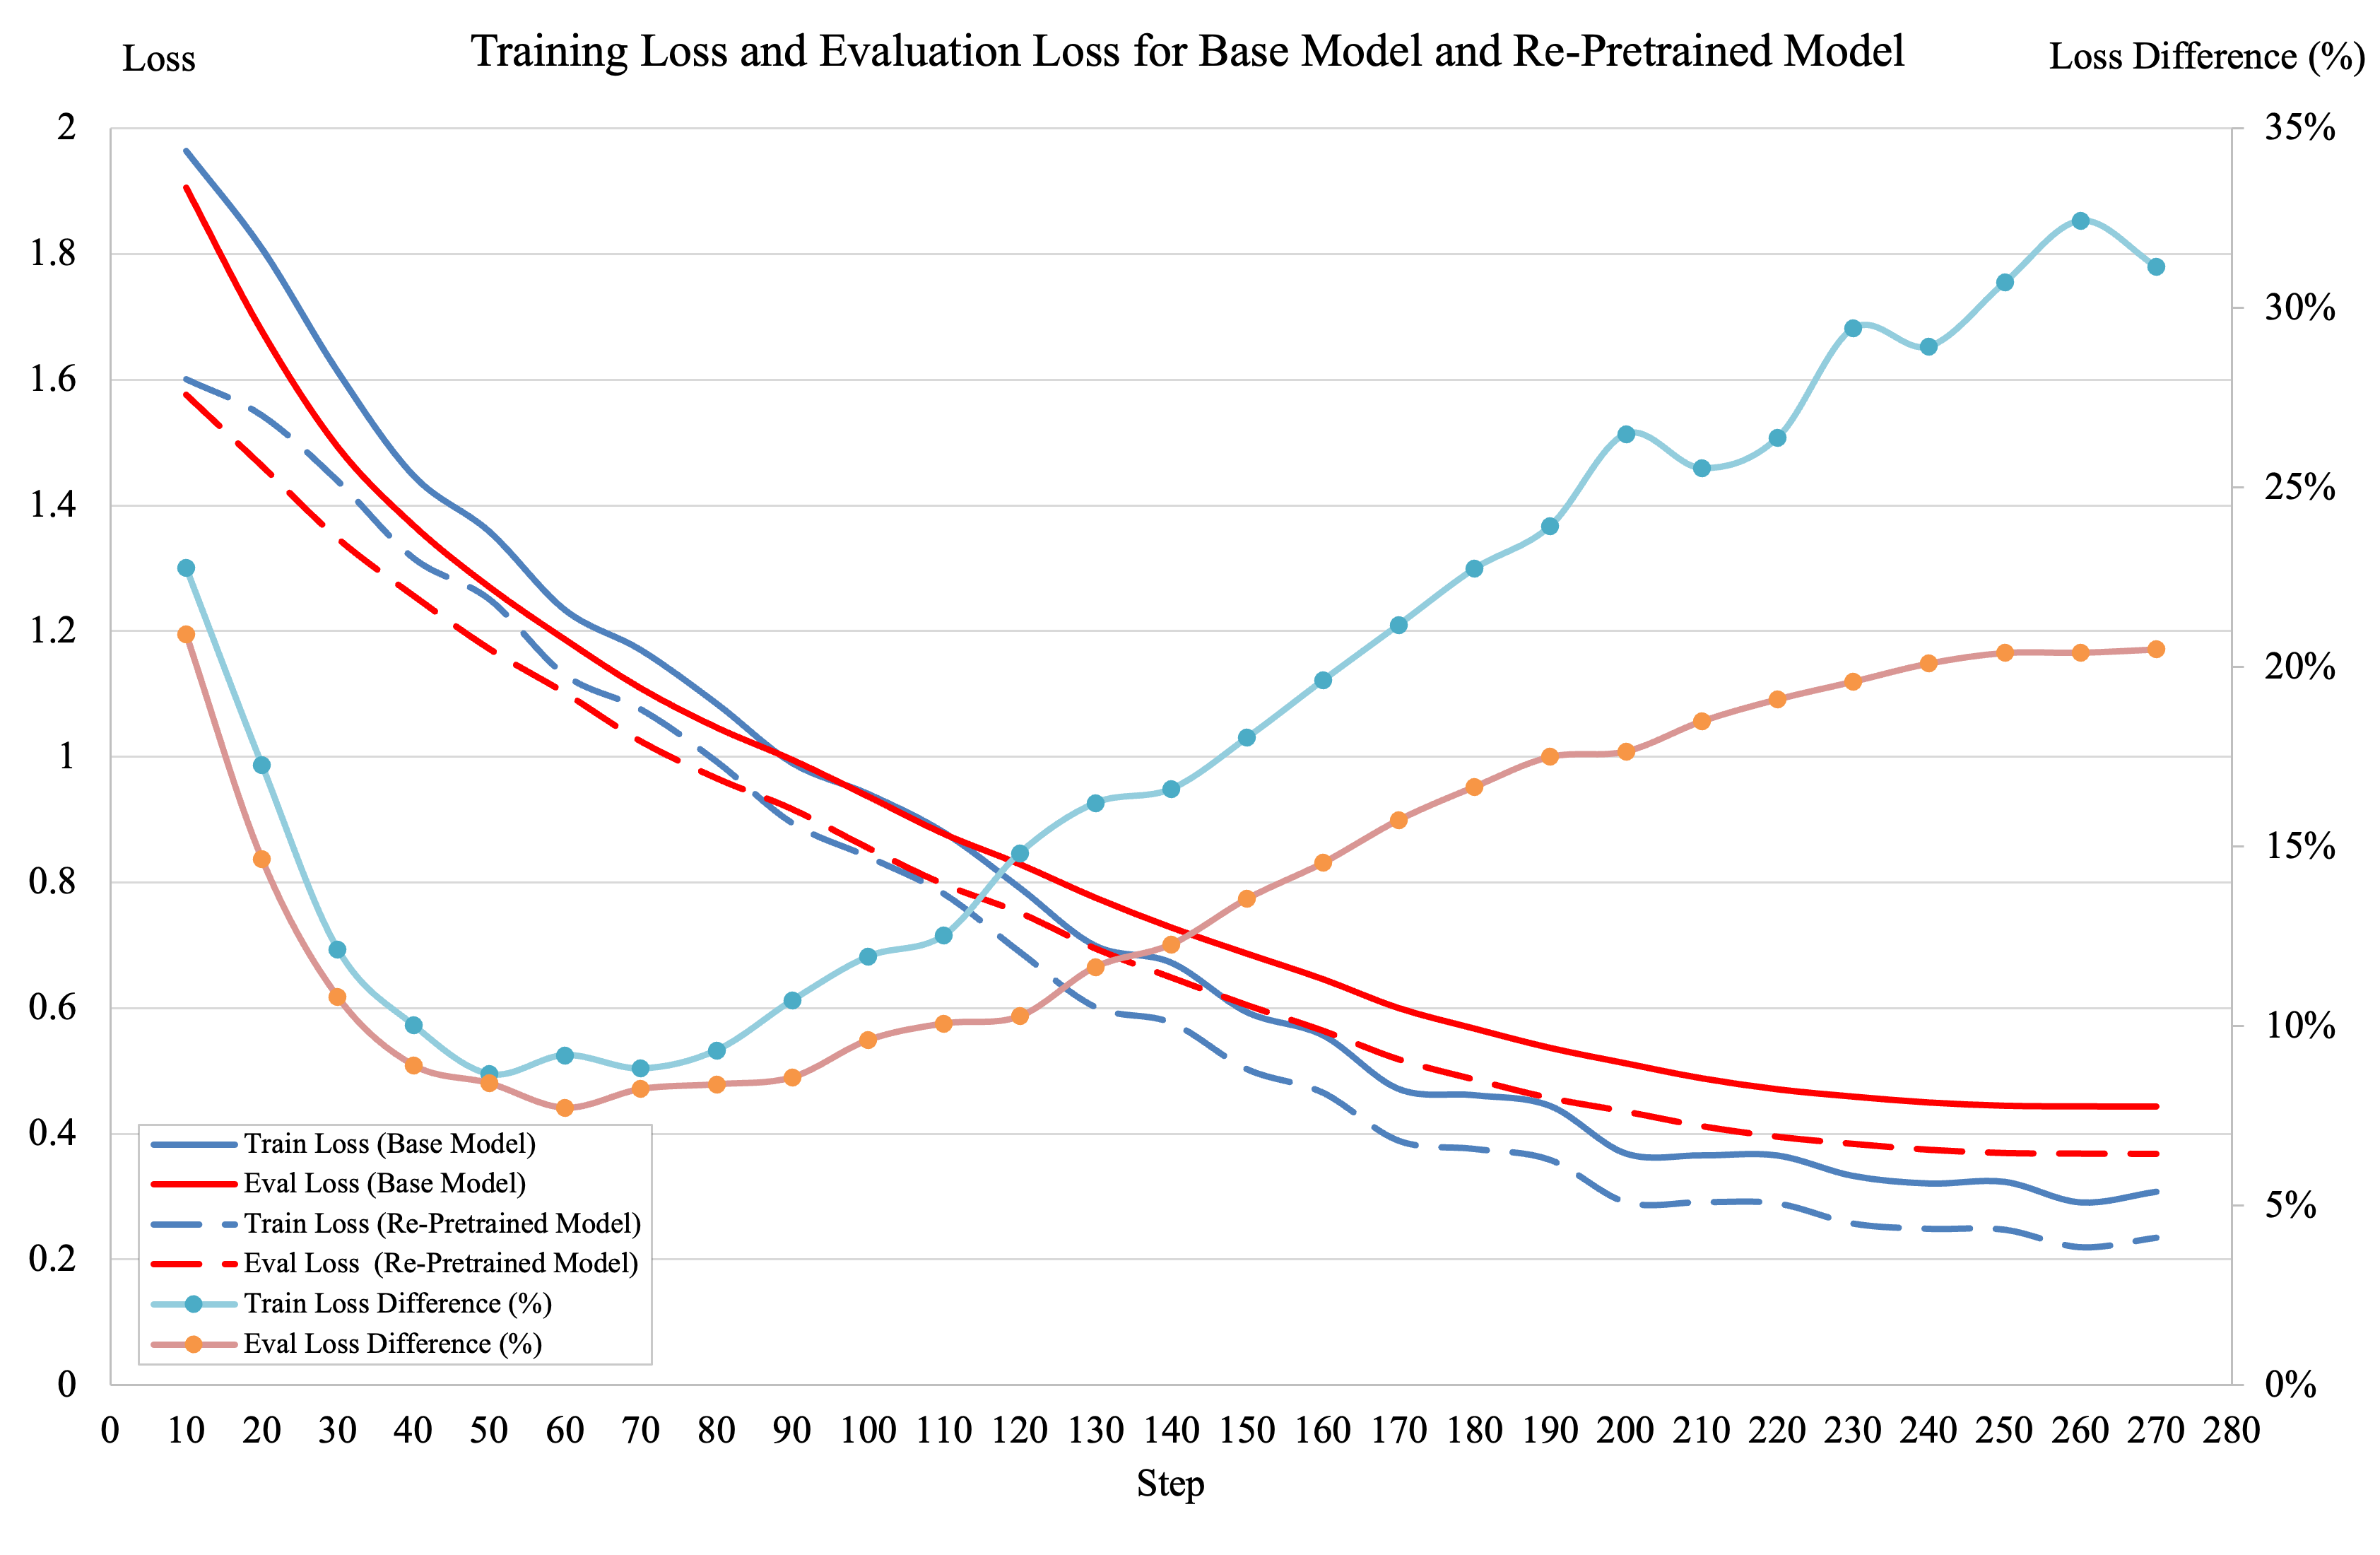
\includegraphics[width=0.9\textwidth]{Chapter2/Chapter2Figs/base_pretrain_loss.png}
            \caption{Training Losses and Evaluation Losses for Base Model and Re-Pretrained Model}
            \label{fig:ch2:training_loss_compare}
    \end{center}
\end{figure}


To sum up, these loss metrics suggest that the model successfully absorbed knowledge from the training data. The observed reduction in both training and evaluation losses over the course of training indicates an improvement in the model's ability to generate required texts. It's worth noting that the model's capacity to reduce the training evaluation loss, despite being trained solely on the training dataset, is indicative of its improved understanding and extrapolation of the underlying patterns for the evaluation dataset.





\section{Evaluating Model Performance}
% To evaluate whether our fine-tuned model can generate consistent results as the target Minutes. In this section, we will outline the approaches used to assess the effectiveness of our fine-tuned model in generating consistent and contextually accurate FOMC Minutes. 

% % 
% % linguistic similarity, contribution of the prompts, statistically significant

% % Levenshtein Similarity Ratio
% % Semantic Similarity metrics

% Evaluating the LLM's performance involves several aspects and different methods. Generally, there are two kinds of metrics, reference-based evaluation and reference-free evaluation. Firstly, the reference-based evaluation compared the model's outputs with the target outputs. Scores are used to measure the difference. Before the 




% According to the literature, we suggest to evaluate the model in three aspects, 1) linguistic similarity, 2) contribution of the prompts, 3) statistically significant. 


% In this section, we will evaluate the performance of the fine-tune LLM. As the nature of the LLM is a probability model, which choose the next token with the highest probability. Therefore, a critical issue involved in the results is the LLM Hallucination. It refers to that the content generated by the model is not supported or confile with the facts. \cite{huang2025survey} have defined two types of Hallucination in LLM, factuality hallucination and faithfulness hallucination. Factuality hallucination refers to the conflict between the generated contents and the real-world facts, while faithfulness hallucination involved if the generated content is not consistent with the inputs. Therefore, Hallucination Detection tests are necessary for the model. 


In this section, we evaluate the performance of the fine-tuned Large Language Model (LLM). Given that an LLM is inherently a probabilistic model, which selects the next token based on the highest probability, a critical issue encountered is the phenomenon known as hallucination. Hallucination refers to instances where the content generated by the model is unsupported by or conflicts with factual information. \cite{huang2025survey} have identified two primary forms of hallucination in LLMs: factuality hallucination and faithfulness hallucination. Factuality hallucination occurs when generated content contradicts real-world facts, whereas faithfulness hallucination arises when the generated content does not align consistently with the provided input. Consequently, tests designed to detect hallucinations are essential for evaluating the reliability of LLMs.


For our research, we applied three types of tests for our model:  1) textual similarity of outputs, 2) contribution of the input prompts, 3) decision making accuracy. 

The first two tests focus on detecting the faithfulness hallucination of the model. Both the textual similarity and the prompts contribution can provide quantitative measures of the overlap of key facts between the generated texts and the given texts. 



% ROGUE
% Firstly, n-gram

% decision 


% Cosine Similarity
Firstly, the textual similarity focuses on comparing the similarity between the target output and the generated output using mathematical distance, such as the Levenshtein Similarity Ratio (\cite{levenshtein1966binary}) and Cosine Similarity (\cite{tanguy2016natural}). The Levenshtein Similarity Ratio replies on the Levenshtein Distance to measure the minimum number of strings that need to be edited from the generated output to the required output. Furthermore, some other metrics driven from the idea of ``n-grams'', such as the Recall-Oriented Understudy for Gisting Evaluation score (ROGUE score, \cite{lin2004rouge}), provide an grammatical-level measurement than the word-level Levenshtein Similarity Ratio. These methods are useful at the age of ``Bag-Of-Word (BOG)''.


% TODO: rogue calculation??


However, with the development of LLM, researchers can take advantage of the embeddings from the LLM rather than the one-hot key of ``BOG''. The embeddings can convert the ``word'' into tokens that encoded more semantic information than the one-hot key. Therefore, the Cosine Similarity provides a more accurate estimation of the semantic similarity between two texts. Here, we will use the Cosine Similarity as our first metric to evaluate the text similarity of outputs. Cosine Similarity ranges from 0 to 1, where a value of 1 indicates a perfect similarity between the two texts, while a value of 0 signifies that the texts are highly different from each other.

The metric helps in determining how well the generated text aligns with the expected content in terms of both meaning and context. For example, \cite{aynetdinov2024semscore}, \cite{kim2024comparison}, and \cite{yauney2023data} used the Cosine Similarity as a benchmark when evaluating the LLM's performance. 


Cosine similarity is estimated by the cosine of the angle between two non-zero vectors. It is defined as the dot product of the two vectors divided by the product of their magnitudes. This mathematical operation helps in quantifying how closely the generated text aligns with the target text in terms of meaning and content. We utilize the ``tokenizer'' from the LLAMA3 model to convert the response texts into vector representations, denoted as $Y_{target}$ for the target text and $Y_{generated}$ for the generated text. The cosine similarity score, denoted as $Cos_{Y_{target}, Y_{generated}}$, is then calculated as follows:


\begin{equation*}
    Cos_{Y_{target}, Y_{generated}} = \frac{Y_{target} \cdot Y_{generated}}{|Y_{target}| |Y_{generated}|}
\end{equation*}


% According to the distribution theory, 
Drawing from distributional semantics theory, which posits that words with similar meanings tend to occur in similar contexts and thus have similar distributions in the vector space, we hypothesize that texts with higher semantic likeness will exhibit a greater cosine similarity. This theory, first proposed by \cite{firth1957linguistics} and later expanded upon in the context of distributional semantics by \cite{sahlgren2008distributional}, suggests that words can be represented as real-valued vectors that encapsulate their linguistic meanings. Consequently, we formulate our hypothesis as follows:

\begin{equation*}
    H0:\quad Cos^{FT} > Cos^{Base}
\end{equation*}

This hypothesis asserts that the cosine similarity score ($Cos_{FT}$) between the target text  and the response generated by the fine-tuned model will be higher than the cosine similarity score ($Cos_{Base}$) between the target text and the response generated by the base model. This expectation is drawn from the assumption that the fine-tuned model, having been specifically optimized for the task at hand, will produce responses that are semantically closer to the target texts compared to the base model. 


% BERTScore 







% Shapley Value

Then, we expect the generated output to contain sufficient information and analysis directly derived from the input prompts rather than relying on the model's imagination. To evaluate this, our second metric assesses the contribution of the key prompts to the generated output. Specifically, we employ the Shapley Value (\cite{shapley1953value}) for this evaluation. The Shapley Value, first came up with game theory, is designed to determine the contribute of each player in a group in a coalitional game. Several researchers introduced and modified the method in studying the the marginal contribution of each prompt to the generated response, ensuring that the model effectively incorporates all relevant information from the input prompts, such as the Shapley Regression Value (\cite{lipovetsky2001analysis}), Shapley Sampling Value (\cite{vstrumbelj2014explaining}), Quantitative Input Influence (\cite{datta2016algorithmic}), and Shapley Additive Explanations (\cite{lundberg2017unified})


% % change to SHAP

The Shapley Value ($\mathcal{SV}$) in LLMs (\cite{liu2023prompt}, \cite{mohammadi2024wait}, \cite{goldshmidt2024tokenshap}) will help answer the question \textit{``\textcolor{blue}{Which input tokens most influenced the model's output?}''} by measuring the expectation of marginal contribution of prompted tokens to the generated tokens:

\begin{equation*}
  \mathcal{SV}_i(f) = \sum_{\mathcal{S} \subset \mathcal{P}\setminus p_i} \frac{\left|\mathcal{S}\right|! (n - \left|\mathcal{S}\right| - 1)!}{n!} \left(f(\mathcal{S}\cup p_i) - f(\mathcal{S})\right)
\end{equation*}

where $\mathcal{P} = {p_1, p_2, \cdots, p_n}$ is the set of prompts. $\mathcal{S}$, also known as coalition, is a subset of $\mathcal{P}$. $\left|\mathcal{S}\right|$ is the number of elements in subset $S$. $\mathcal{f}(\mathcal{S})$ represents the output from the LLM $f(\cdot)$ given the prompts $\mathcal{S}$. Then, \textcolor{red}{the marginal contribution of prompt $p_i$ to the output is calculated by $f(\mathcal{S} \cup p_{i}) - \mathcal{f}(\mathcal{S})$}. Here, we followed the approach of \cite{lundberg2017unified} and \cite{goldshmidt2024tokenshap} and compared the differences at the token level using Cosine Similarity.

To calculate the Shapley Value, we first masked the data ($p_i$) in the prompts, such as the Federal Efficient Rate, Unemployment Rate, Yield Curve, and etc. Then we ask the model to generate the response based on the masked prompt ($f(\mathcal{S})$). We set the response without mask prompt as our base value ($f(\mathcal{S}\cup p_i)$) and calculate the Cosine Similarity as our score. Because we need the response to provide sufficient analysis of the economic and financial information. \textcolor{red}{When prompts are masked, the marginal contribution should be positive.} A large positive Shapley Value indicates that the masked prompt significantly influences the LLM's output.


% decision making accuracy 
Finally, to detect the Factuality Hallucination, we focus on the committee voted actions. As the committee need to vote for the monetary policy especially the level of the Federal Effective Rate, we compare the decisions made by the model and the facts. 





Lastly, we will conduct significance tests on the generated texts to statistically validate the improvements brought about by the fine-tuning process. 
% These tests will help in confirming whether the observed enhancements in text generation are statistically significant and not due to random variations.


% By combining these evaluation methods, we aim to provide a robust assessment of the model's performance, highlighting its strengths and identifying areas for further improvement.






\section{Empirical Results}\label{ch2:sec:empirical results}

In this section, a comparative analysis was conducted to evaluate the performance of our fine-tuned model (FT Model) against the unmodified model (Base Model) in the context of generating Federal Open Market Committee (FOMC) Minutes. This comparison aimed to highlight the improvements achieved through the fine-tuning process, specifically focusing on the model's ability to capture the nuances and complexities inherent in the FOMC Minutes' content and style.

The results of this comparison provided insights into the effectiveness of our prompting and fine-tuning strategy, demonstrating the model's enhanced understanding and generation capabilities specifically tailored to the domain of FOMC Minutes. 

\subsection{Generating Results}

Firstly, Section \ref{target_text} is the target texts extracted from the 20191030 FOMC Minutes. Applying our CoT prompting, Section \ref{ft_model} demonstrates the results for Fine-tuned model, while Section \ref{base_model} shows the results for the base model. Finally, Section \ref{simualted ft} gives an example using the simulated data (here we use S\&P 500 index return) to generate the ``Staff Review of Financial Situation'' in the FOMC Minutes. A well-structured synthetic FOMC Minutes is provided in the Appendix \ref{app:fomc 20191030} (FOMC Minutes for 20191030), Appendix \ref{app:fomc simuated summary} (Summary FOMC Minutes with simulated equity data), and Appendix \ref{app:fomc simuated} (Full FOMC Minutes Chapter with simulated equity data)



\subsection{Raw Model Results}
% ## TODO: add FOMC generated by raw model





\subsection{Fine-tuned Model Results}

\subsubsection{Target Text: From Data to Staff Economic Outlook for FOMC Minutes 20191030}\label{target_text}

\textbf{User Prompt:}\\
{\footnotesize
\textit{
Please write a summary of section "Staff Review of the Economic Situation" based the given data for 20091030: \\
\textcolor{red}{'cpi growth rate for the year': -0.009779758,0.036015062,0.045381515,0.045116153,0.002961999,-0.003901354,0.027694514,0.01097724,0.018466153,0.033927388,}\\
'fed\_funds\_rate for the month': 1.83, \\
'Annualized GDP growth rate for the year': -0.048549963, -0.013766568, 0.018815073, 0.056022881, \\
'mortgage\_rate for the month': 3.65, 3.57, 3.69, 3.75, 3.78, \\
'unemployment rate for the year': 4,3.8,3.8,3.7,3.6,3.6,3.7,3.6,3.5,3.6}
}\\
\textbf{Target Text:}\\
{\footnotesize
\textit{
    - **GDP Growth:** Revised down slightly for the second half of 2019. Real GDP forecasted to decelerate modestly over the medium term.\\
    - \textcolor{red}{**Inflation:** Core PCE inflation forecasted to remain below 2\% through 2022.}\\
    - **Risks:** Risks to GDP growth seen as tilted to the downside due to global trade tensions and weak business investment.
}}\\
~\\
\textbf{User Prompt:}\\
{\footnotesize
\textit{
Please write a summary of section "Staff Review of the Financial Situation" based the given data for 20091030: \\
'10-year yield rate mines 2-year yield rate for the month': 0.09, 0.12, 0.15, 0.12, 0.1, 0.12, 0.12, 0.14,0.13, ., 0.16, 0.17, 0.16, 0.18, 0.18, 0.18,0.19, 0.19, 0.17, 0.21, 0.2, 0.17, 0.17, \\
'S\&P 500 Index return': 0.33\%,-0.08\%,0.56\%,0.41\%,0.19\%,0.28\%,-0.36\%,0.69\%,-0.39\%,0.28\%,-0.20\%,1.00\%,-0.14\%,1.09\%,0.64\%,0.91\%,-1.56\%,-0.45\%,1.42\%,0.80\%,-1.79\%,-1.23\%.}
}\\
\textbf{Target Text:}\\
{\footnotesize
\textit{
    - **Investor Sentiment:** Initially weakened but later strengthened on favorable trade and Brexit news. Equity prices and corporate bond spreads remained stable.\\
    - **Short-term Funding:** Volatility in U.S. short-term funding markets was alleviated by the Desk's repo operations.\\
    - **Global Markets:** Financial conditions improved after initial concerns; the dollar index declined slightly.\\
    - **Corporate Financing:** Conditions remained generally accommodative, with mixed results in issuance and borrowing.\\
    - **Housing Market:** Mortgage rates remained low, leading to stable home-purchase originations and increased refinancing activity.\\
    - **Consumer Credit:** Financing conditions supportive of household spending, though tight for nonprime credit scores.\\
}}\\
~\\
\textbf{User Prompt:}\\
{\footnotesize
\textit{
    Please write a summary of section "Staff-Economic-Outlook" based the above sections.
}}\\
\textbf{Target Text:}\\
{\footnotesize
\textit{
    The staff revised down its GDP growth projections for 2019 to 2.1\% and 2.0\% for 2020 due to weaker-than-expected data. The unemployment rate was projected to remain low, \textcolor{red}{but inflation was expected to stay below the 2\% target}. The risks to the forecast were seen as balanced, with potential upside from fiscal policy and a strong labor market.
}}\\
~\\
\textbf{User Prompt:}\\
{\footnotesize
\textit{Generate the FOMC Minutes Staff-Economic-Outlook Section using the summary you just generated}}\\
\textbf{Target Text:}\\
{\footnotesize
\textit{The projection for U.S. real GDP growth prepared by the staff for the October FOMC meeting was revised down a little for the second half of this year relative to the previous projection.  This revision reflected the estimated effects of the strike at General Motors along with some other small factors. \\
... ...\\
The unemployment rate was projected to be roughly flat through 2022 and to remain below the staff’s estimate of its longerrun natural rate. The staff’s forecast for core PCE price inflation this year was revised down a little in response to recent data.  Beyond this year, the projection for core inflation was unrevised, and the forecast for total inflation was a little lower in 2020 because of a downward revision in projected consumer energy prices.  Both total inflation and core inflation were forecast to move up slightly next year, as the low inflation readings early this year were viewed as transitory; \textcolor{red}{nevertheless, both inflation measures were forecast to continue to run somewhat below 2 percent through 2022.}  \\
... ... \\
The risks to the inflation projection were also viewed as  Federal Open Market Committee having a downward skew, in part because of the downside risks to the forecast for economic activity. }
}

\subsubsection{Fine-Tuned Model: From Data to Staff Economic Outlook for FOMC Minutes 20191030}\label{ft_model}

\textbf{User Prompt:}\\
{\footnotesize
\textit{
Please write a summary of section "Staff Review of the Economic Situation" based the given data for 20091030: \\
\textcolor{red}{'cpi growth rate for the year': -0.009779758,0.036015062,0.045381515,0.045116153,0.002961999,-0.003901354,0.027694514,0.01097724,0.018466153,0.033927388,} \\
'fed\_funds\_rate for the month': 1.83, \\
'Annualized GDP growth rate for the year': -0.048549963, -0.013766568, 0.018815073, 0.056022881, \\
'mortgage\_rate for the month': 3.65, 3.57, 3.69, 3.75, 3.78, \\
'unemployment rate for the year': 4,3.8,3.8,3.7,3.6,3.6,3.7,3.6,3.5,3.6}
}\\
\textbf{FT Model Response:}
{\footnotesize
\textit{
    The U.S. economy continued to expand at a moderate pace. Labor market conditions improved with a strong increase in nonfarm payroll employment and a decrease in the unemployment rate to 3.7\%. Real GDP growth was projected to be moderate in the near term, supported by consumer and business spending. \textcolor{red}{Inflation was expected to stabilize around 2\% over the medium term}.
}}
~\\
\textbf{User Prompt:}\\
{\footnotesize
\textit{
Please write a summary of section "Staff Review of the Financial Situation" based the given data for 20091030: \\
'10-year yield rate mines 2-year yield rate for the month': 0.09, 0.12, 0.15, 0.12, 0.1, 0.12, 0.12, 0.14,0.13, ., 0.16, 0.17, 0.16, 0.18, 0.18, 0.18,0.19, 0.19, 0.17, 0.21, 0.2, 0.17, 0.17, \\
'S\&P 500 Index return': 0.33\%,-0.08\%,0.56\%,0.41\%,0.19\%,0.28\%,-0.36\%,0.69\%,-0.39\%,0.28\%,-0.20\%,1.00\%,-0.14\%,1.09\%,0.64\%,0.91\%,-1.56\%,-0.45\%,1.42\%,0.80\%,-1.79\%,-1.23\%.}
}\\
\textbf{FT Model Response:}\\
{\footnotesize
\textit{
    - **Market Conditions:** Financial conditions were stable, with the federal funds rate remaining unchanged. Equity prices rose, corporate bond spreads narrowed, and interest rates on short-term debt decreased. \\
    - **Monetary Policy Expectations:** Market participants anticipated a rate cut in September and additional cuts later in the year. The federal funds rate futures implied a higher probability of a rate cut in July and September. \\
    - **Global Financial Conditions:** Global financial conditions were mixed, with increased concerns over trade tensions and economic growth in some countries. Financial conditions in emerging markets remained strained, particularly in Turkey and Argentina. \\
    - **Consumer and Business Financing:** Consumer credit expanded at a solid pace, with increases in credit card and auto loans. Business financing conditions remained supportive, with solid credit quality.
}}\\
~\\
\textbf{User Prompt:}\\
{\footnotesize
\textit{
    Please write a summary of section "Staff-Economic-Outlook" based the above sections.
}}\\
\textbf{FT Model Response:}\\
{\footnotesize
\textit{
    The staff revised down its GDP growth projections for 2019 to 2.1\% and 2.0\% for 2020 due to weaker-than-expected data. The unemployment rate was projected to remain low, \textcolor{red}{but inflation was expected to stay below the 2\% target}. The risks to the forecast were seen as balanced, with potential upside from fiscal policy and a strong labor market.
}}
~\\
\textbf{User Prompt:}\\
{\footnotesize
\textit{Generate the FOMC Minutes Staff-Economic-Outlook Section using the summary you just generated}}\\
\textbf{FT Model Response:}\\
{\footnotesize
\textit{
In the economic forecast prepared for the September FOMC meeting, the staff revised down its projection for real GDP growth in the second half of 2019.  The staff’s forecast for the second half of the year was based on a number of factors, including a more negative assessment of foreign economic growth and a slightly weaker outlook for the U.S. business sector.  The staff’s projection for real GDP growth over the medium term was little changed.  The staff continued to project that real GDP would decelerate modestly over the medium term, reflecting the expected gradual decline in fiscal policy stimulus and the staff’s assumption that the effects of monetary policy on the economy would become less accommodative.  The staff continued to forecast that the unemployment rate would decline further and that the labor market would tighten further, although at a slower pace than in recent years. \\
... ... \\
\textcolor{red}{The staff’s forecast for the unemployment rate over the medium term was little changed.  The staff’s projection for core PCE inflation was little changed, as the staff continued to expect that inflation would remain below 2 percent through 2022.}  The staff’s projection for total PCE price inflation was also little changed, as the staff continued to expect that gasoline prices would be volatile and that inflation would run a bit below core inflation.}
}

\subsubsection{Base Model Response: From Data to Staff Economic Outlook for FOMC Minutes 20191030}\label{base_model}

\textbf{User Prompt:}\\
{\footnotesize
\textit{
Please write a summary of section "Staff Review of the Economic Situation" based the given data for 20091030: \\
\textcolor{red}{'cpi growth rate for the year': -0.009779758,0.036015062,0.045381515,0.045116153,0.002961999,-0.003901354,0.027694514,0.01097724,0.018466153,0.033927388,} \\
'fed\_funds\_rate for the month': 1.83, \\
'Annualized GDP growth rate for the year': -0.048549963, -0.013766568, 0.018815073, 0.056022881, \\
'mortgage\_rate for the month': 3.65, 3.57, 3.69, 3.75, 3.78, \\
'unemployment rate for the year': 4,3.8,3.8,3.7,3.6,3.6,3.7,3.6,3.5,3.6}
}\\
~\\
\textbf{Base Model Response:}\\
{\footnotesize
\textit{
    Based on the provided data, here is a summary of the "Staff Review of the Economic Situation":\\
    The data appears to be a review of the economic situation for the year ending 20091030. The review includes several key economic indicators:\\
    * CPI growth rate: \textcolor{red}{The Consumer Price Index (CPI) growth rate for the year was -0.0098, -0.0360, 0.0454, 0.0451, and 0.0029, indicating a decline in inflation in the early part of the year, followed by a slight increase later on.}\\
    ... ...\\
    Overall, the review suggests that the economy experienced a decline in inflation and economic growth in the early part of the year, followed by a slight increase later on. Mortgage rates and unemployment rates also showed some fluctuations over the year.
}}\\
~\\
\textbf{User Prompt:}\\
{\footnotesize
\textit{
Please write a summary of section "Staff Review of the Financial Situation" based the given data for 20091030: \\
'10-year yield rate mines 2-year yield rate for the month': 0.09, 0.12, 0.15, 0.12, 0.1, 0.12, 0.12, 0.14,0.13, ., 0.16, 0.17, 0.16, 0.18, 0.18, 0.18,0.19, 0.19, 0.17, 0.21, 0.2, 0.17, 0.17, \\
'S\&P 500 Index return': 0.33\%,-0.08\%,0.56\%,0.41\%,0.19\%,0.28\%,-0.36\%,0.69\%,-0.39\%,0.28\%,-0.20\%,1.00\%,-0.14\%,1.09\%,0.64\%,0.91\%,-1.56\%,-0.45\%,1.42\%,0.80\%,-1.79\%,-1.23\%.}
}\\
\textbf{Base Model Response:}\\
{\footnotesize
\textit{
    Based on the provided data, here is a summary of the "Staff Review of the Financial Situation":\\
    The data appears to be a review of the financial situation for the year ending 20091030. The review includes several key financial indicators:\\
    * 10-year yield rate vs. 2-year yield rate: The spread between the 10-year yield rate and the 2-year yield rate was 0.09, 0.12, 0.15, 0.12, 0.1, 0.12, 0.12, 0.14, 0.13, and so on, indicating a fluctuation in the yield curve over the year.\\
    ... ...\\
}}\\
~\\
\textbf{User Prompt:}\\
{\footnotesize
\textit{
    Please write a summary of section "Staff-Economic-Outlook" based the above sections.
}}\\
\textbf{Base Model Response:}\\
{\footnotesize
\textit{
    Based on the provided data, here is a summary of the "Staff-Economic-Outlook":\\
    The "Staff-Economic-Outlook" section appears to be a summary of the economic outlook based on the previous sections. Here are the key points:\\
    * Economic growth: The outlook suggests that the economy experienced a decline in economic growth in the early part of the year, followed by a slight increase later on. The annualized GDP growth rate was -0.0485, -0.0138, and 0.0188, indicating a decline in economic growth in the early part of the year, followed by a slight increase later on.\\
    * Inflation: The outlook suggests that inflation was declining in the early part of the year, but then increased slightly later on. \textcolor{red}{The CPI growth rate was -0.0098, -0.0360, 0.0454, 0.0451, and 0.0029, indicating a decline in inflation in the early part of the year, followed by a slight increase later on.}\\
    ... ...
}}\\
~\\
\textbf{User Prompt:}\\
{\footnotesize
\textit{Generate the FOMC Minutes Staff-Economic-Outlook Section using the summary you just generated}}\\
\textbf{Base Model Response:}\\
{\footnotesize
\textit{
    *Staff-Economic-Outlook**\\
The staff's economic outlook is characterized by a slow recovery in the early part of the year, followed by a slight increase in economic growth and inflation later on. The annualized GDP growth rate has declined in the early part of the year, but has since stabilized and shown signs of improvement. \textcolor{red}{The CPI growth rate has also declined in the early part of the year, but has since edged up slightly.} \\
... ... 
}}\\
~\\



Compared with the based model, the fine-tuned model capitalizes on the enriched training dataset, which specialized in economic and financial analysis. Consequently, the fine-tuned model not only excels in mirroring the format of the target texts more accurately but also demonstrates an enhanced capability to synthesize and analyze data meaningfully within the generated content. In contrast, the base model primarily focuses on recounting the provided data, lacking the nuance and analytical depth that the fine-tuned variant exhibits. For instance, in the evidence of the model's treatment of inflation rates, as measured by Consumer Price Indices (CPIs), the fine-tuned model adeptly captures the dynamics of rising inflation, predicting that the Federal Reserve will try to maintain the inflation rate at a relatively subdued level, targeting around 2\%.

The qualitative comparison in performance from the base model to the fine-tuned model is indicative of the latter's readiness for practical applications in generating FOMC Minutes. The fine-tuned model's outperforming in replicating the style, structure, and analytical content of official documents positions it as a valuable tool in simulating or analyzing potential outcomes of FOMC deliberations. 


\subsubsection{Fine-tuned Model Response: Simluated Data to Staff Review of Financial Situation for FOMC Minutes 20191030}\label{simualted ft}
\textbf{User Prompt:}\\
{\footnotesize
\textit{
Please write a summary of section "Staff Review of the Financial Situation" based the given data for 20191030: \\
'Daily S\&P 500 Index return for the month': 'S\&P 500 Index return':'0.05\%', '-1.09\%', '-0.67\%', '1.18\%', '0.06\%', '-0.06\%', '0.22\%', '0.81\%', '0.44\%', '-0.16\%', '0.94\%', '-0.35\%', '0.67\%', '0.70\%', '\textcolor{red}{-0.11\%', '0.13\%', '0.17\%', '0.70\%', '0.40\%', '0.64\%', '0.83\%'}}
}\\
\textbf{FT Model Response:}\\
{\footnotesize
\textit{
    - **Financial Markets:** Financial conditions remained generally accommodative despite some fluctuations. Stock prices rose, and concerns over the trade tensions eased slightly.
    - **Short-Term Funding Markets:** Market participants reported stable short-term funding conditions, with an increase in overnight repo usage.
    - **Equity and Credit Markets:** \textcolor{red}{Equity prices rose,} and credit conditions for nonfinancial firms remained favorable. Corporate bond issuance remained robust, with strong demand for high-yield bonds.
    - **Global Financial Conditions:** \textcolor{red}{Global financial conditions remained generally supportive of growth}. The U.S. dollar depreciated against most major currencies, and emerging market equity prices increased.
}}\\
~\\
\textbf{Base Model Response:}\\
{\footnotesize
\textit{
The staff review of the financial situation highlighted that the financial markets experienced a mixed performance in the past month. \textcolor{red}{The staff noted that the index experienced a series of small gains and losses, with no clear trend emerging.} Overall, the financial markets were characterized by a lack of direction and volatility in the past month.
}}\\



In this example, we employed a simulated upward sloping curve for the S\&P 500 index returns. The fine-tuned model exhibited a commendable ability to discern and reflect this trend accurately in its generated text. Conversely, the base model fell short in recognizing and articulating the upward trajectory, which highlights the disparity in analytical prowess between the two models. 

Our initial findings indicated that while the model could produce outputs that resemble the intended format and style. However, the overall quality and accuracy of the responses were yet to reach optimal levels. As mentioned before, our training loss is still reducing, which has not been converged to a stable level. This gap in performance underscores the need for further refinements in our fine-tuning approach.



The performance of the fine-tuned model is contingent upon the quality and relevance of the training dataset. To address these shortcomings and elevate the model's capabilities, we propose a two ways to resolve the problem. Enhanced text cleaning, firstly, is a more rigorous preprocessing phase will be implemented to ensure that the target texts are free from noise and inconsistencies. This step is pivotal in enabling the model to learn from clean, structured data, thereby improving its comprehension and generation abilities. Additionally, We try to employ Semantic Labeling to facilitate a deeper understanding of the interplay between economic data and the corresponding narrative. More specifically, we plan to annotate key terms and phrases within the target texts. This labeling process will assist the model in establishing connections between quantitative data and qualitative descriptions, thereby enhancing its capacity to weave data-driven insights into coherent narratives.

However,  the quality of the responses is still not good enough. Therefore, we suggest to two ways to resolve the problem. Firstly, we will conduct a deeper clean in the target texts. Additionally, we will label the important words in the target text to help the model create a connection between the ``data'' and the ``writing''. Futhermore, we will use our supplementary texts, including the Green books an the Blue books, to help the model learning the way of writing. Moreover, we intend to leverage supplementary materials, notably the Green Books and Blue Books, which are integral resources in the Federal Reserve's decision-making process. These documents contain detailed analyses and forecasts, and incorporating them into our training regimen will provide the model with additional context and depth. By learning from these comprehensive texts, the model will gain a richer understanding of the economic landscape and the nuances of crafting authoritative financial reports, ultimately refining its ability to generate high-quality FOMC Minutes.


In summary, by implementing these strategies—enhancing data preprocessing, annotating critical information, and integrating supplementary educational materials, we aim to significantly enhance the fine-tuned model's performance, moving closer to realizing our objective of automating the generation of FOMC Minutes with precision and accuracy.


\subsection{Cosine Similarity Results}

In this section, we calculate the cosine similarity separately for each section, comparing the fine-tuned model with the base model. Converting texts into embedding tokens relies on the tokenizer used. A robust tokenizer can more effectively capture accurate semantic information within the output vectors. Motivated by the methodologies described in \cite{aynetdinov2024semscore} and \cite{zhang2019bertscore}, our research employs two distinct tokenizers for similarity scoring: LLAMA3's tokenizer, pre-trained on a decoder-only model, and BERT's tokenizer, pre-trained on an encoder-only model. Additionally, we incorporate the ROUGE score from the n-gram literature as an additional comparative metric.


Then, we employ the bootstrapping method by randomly selecting samples from the input. Then we calculate the mean similarity for each sample, and create the Empirical Confidence Interval to evaluate the performance of the models. More specifically, we choose 10 responses out of 60 from the test dataset. Then we calculate the mean of the cosine similarity for these 10 sample responses. We keep repeating selecting the sample from the dataset with replacement for 200 times. We calculate and plot the Confidence Interval for the finally results in Table \ref{tab:ch2:cos_ci} and Figure \ref{fig:ch2:cos_ci}.

\begin{table}[h]
    \scriptsize
    \centering
    \begin{tabular}{c  c c c}
      \toprule
        &Mean & Lower 95\% CI& Upper 95\% CI \\
        \hline
        Base Model& 0.7030& 0.6860& 0.7190\\
        & $(714.78)^{***}$& $(697.43)^{***}$& $(731.07)^{***}$\\
       FT Model& 0.8743& 0.8503& 0.8970\\
        &$(604.05)^{***}$& $(587.55)^{***}$& $(619.78)^{***}$\\
       \bottomrule
    \end{tabular}
    \caption{Confidence Intervals for Cosine Similarity for FT Model and Base Model}
    \label{tab:ch2:cos_ci}
\end{table}


\begin{figure}
    \centering
    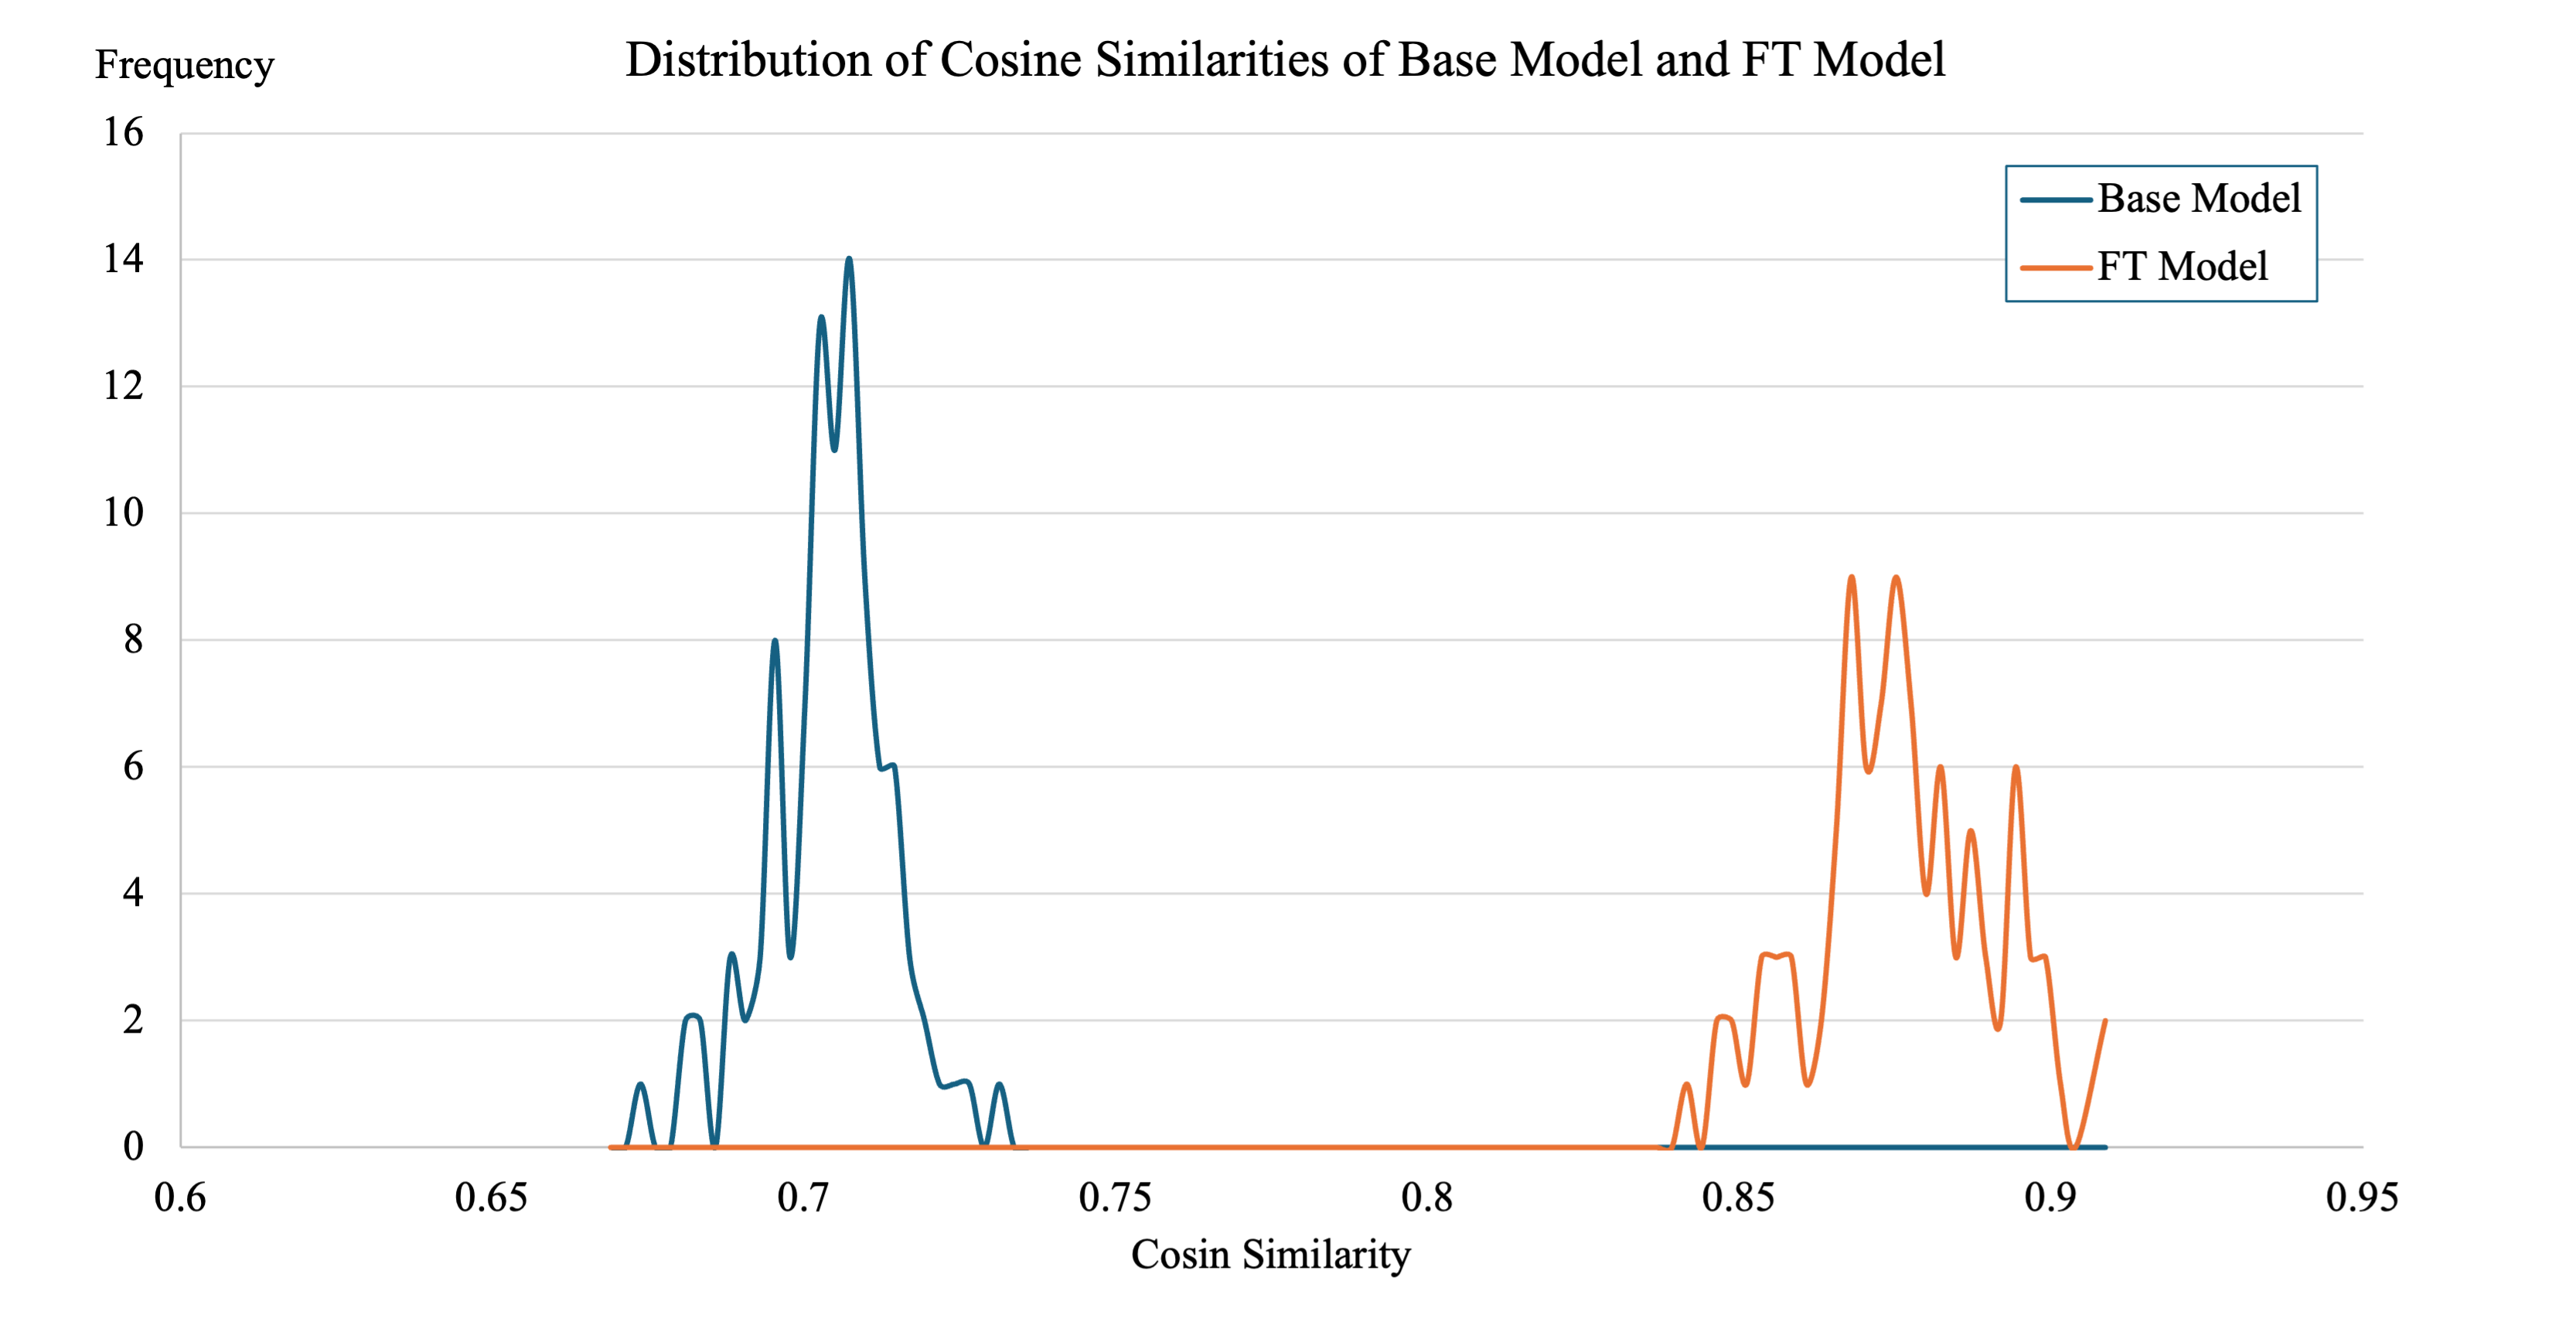
\includegraphics[width=0.8\textwidth]{Chapter2/Chapter2Figs/cos_20250313.png}
    \caption{Cosine Similarity for FT Model and Base Model}
    \label{fig:ch2:cos_ci}
\end{figure}

The reported Cosine Similarity for the fine-tuned model (mean 0.8743 and significant at 99\% level) is much larger than that of the base model (mean 0.7030 and significant at 99\% level). Thus, it can be concluded that our fine-tuning process has been successful in enhancing the model's ability to generate responses that are more consistent and contextually relevant to the input texts. This outcome highlights the effectiveness of the fine-tuning strategy in tailoring the model's output to better suit specific tasks or domains, thereby improving its overall utility and performance.





\subsection{Shapley Value Test}
% TODO: add results about shapley here!!!




\begin{figure}
    \centering
    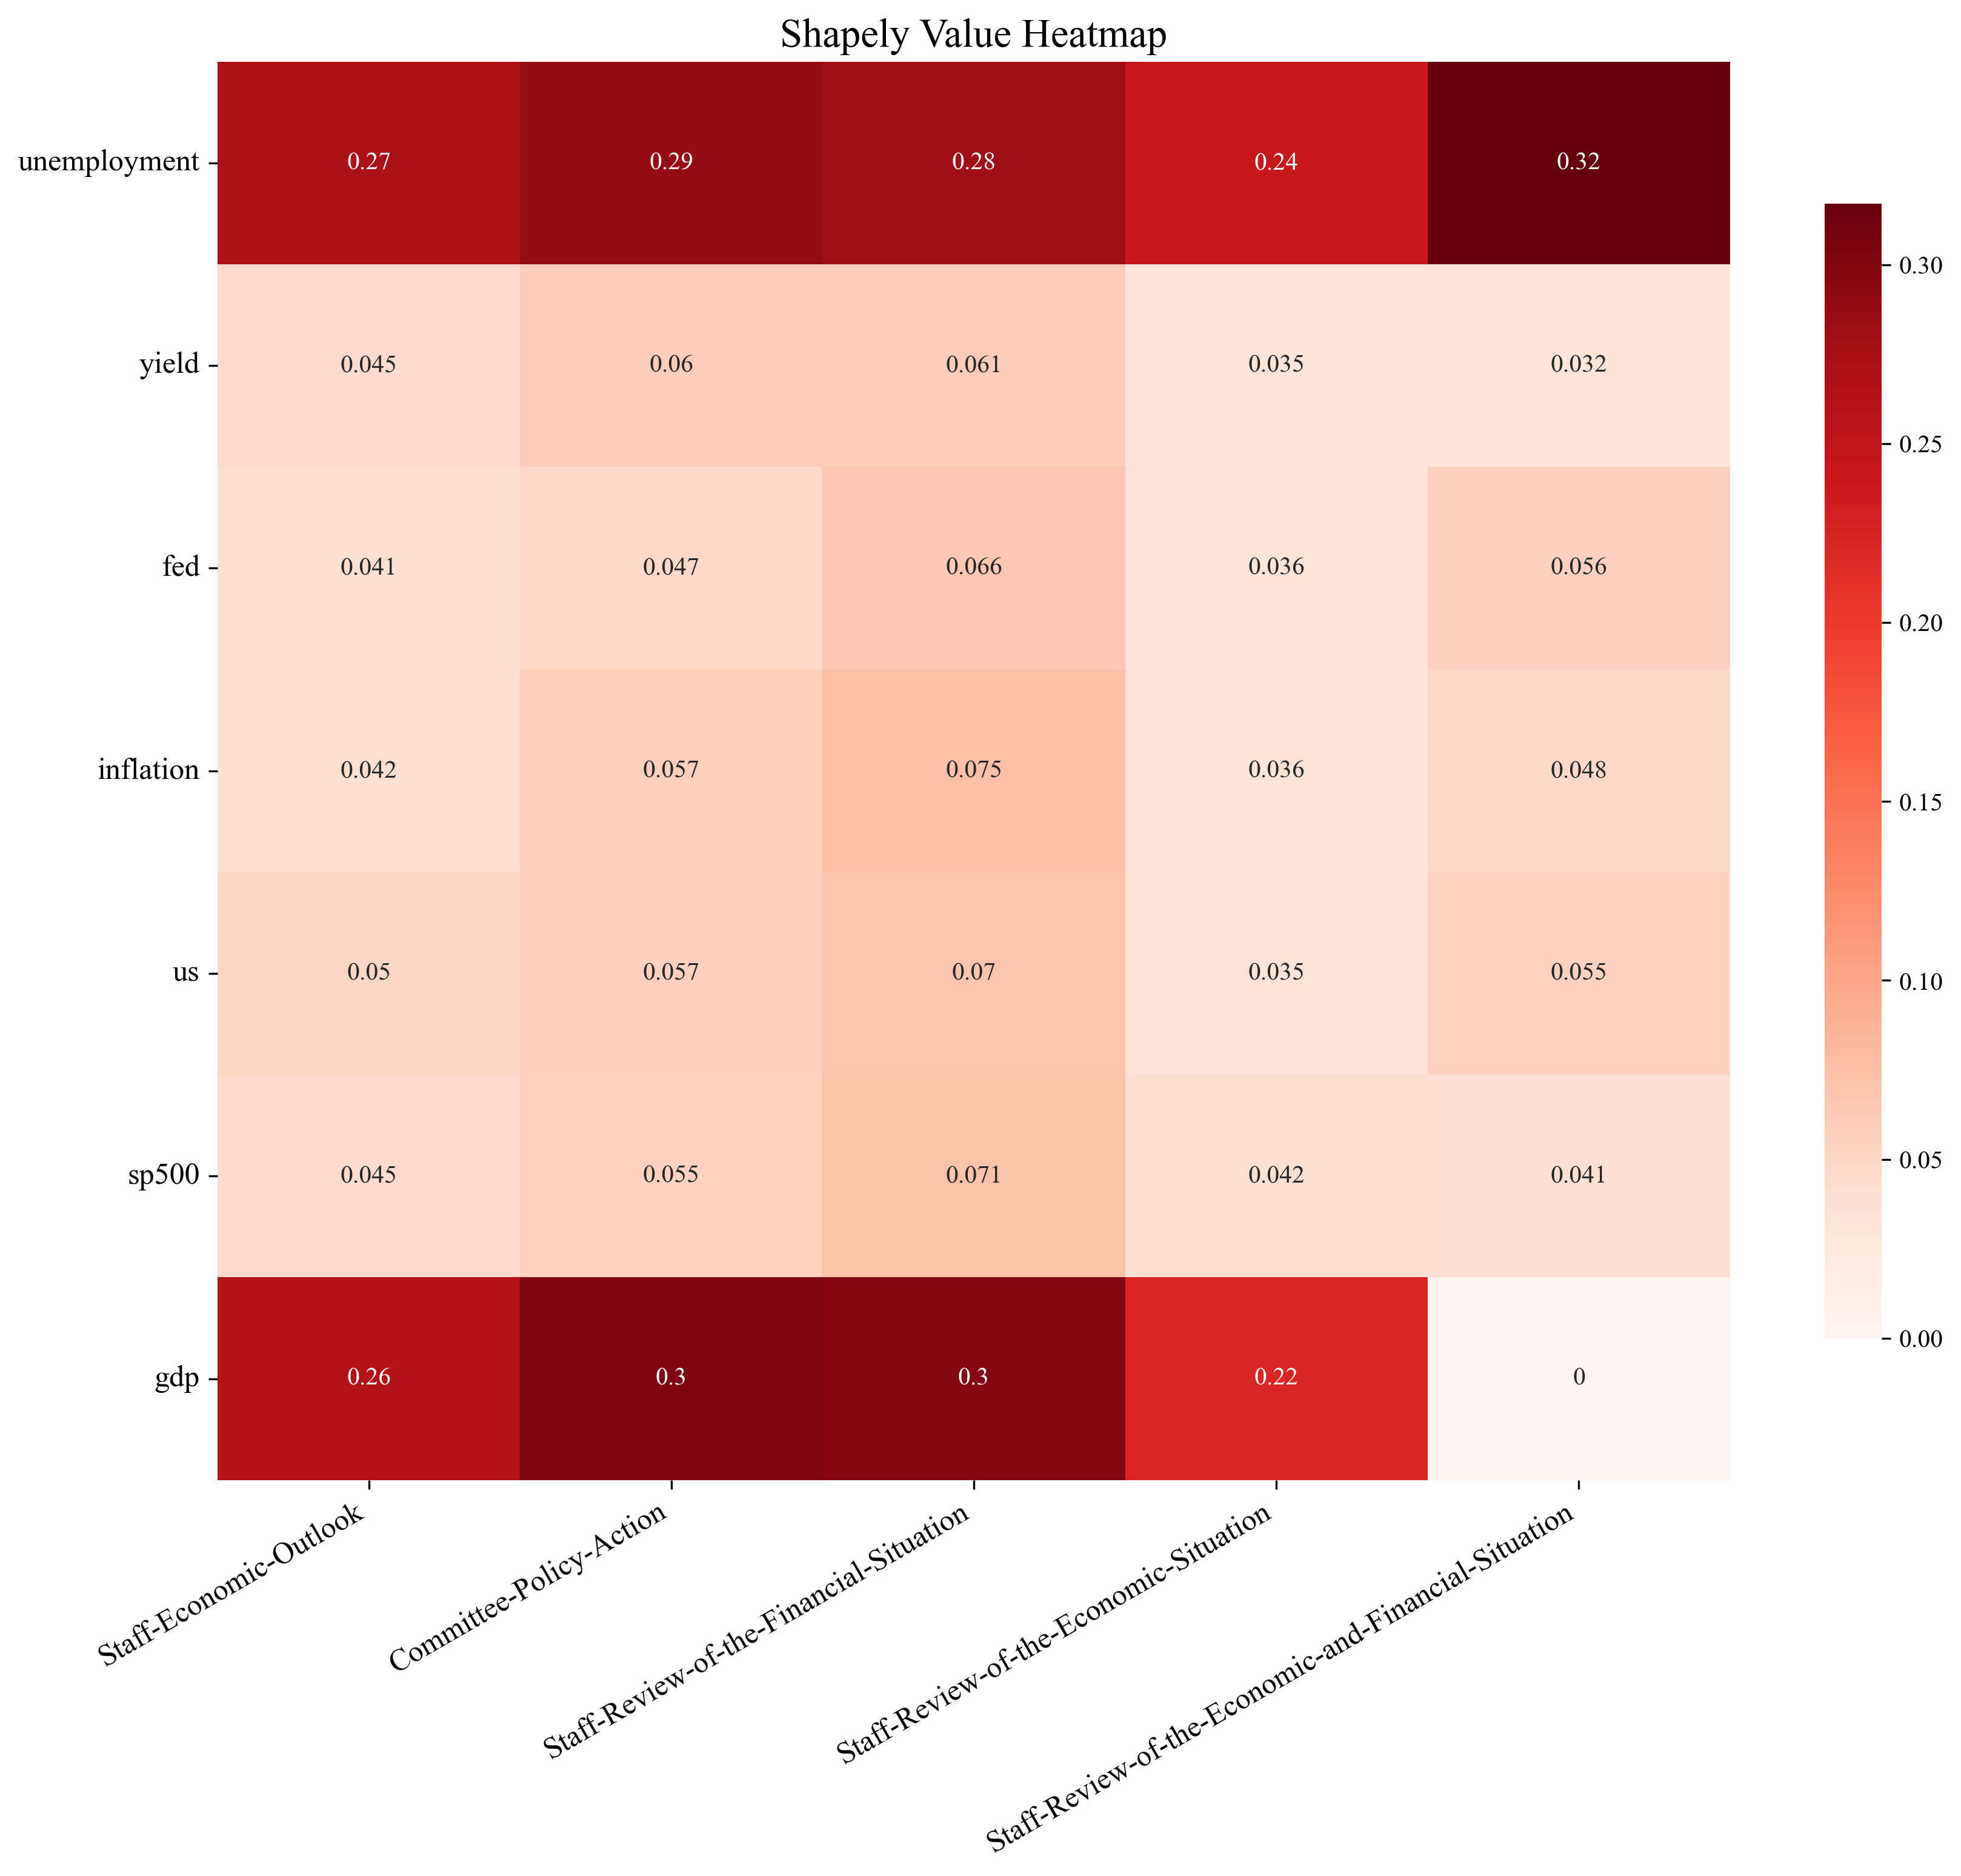
\includegraphics[width=0.8\textwidth]{Chapter2/Chapter2Figs/cos_heatmap_20250313.png}
    \caption{Shapley Value Heatmap for Sections and Masked Prompts}
    \label{fig:ch2:cos_ci}
\end{figure}







% \cite{lundberg2017unified} first suggests to use the 
% https://github.com/shap/shap


% Furthermore, \cite{lundberg2017unified} introduced an efficient way in 





% As for the utility function $\mathcal{U}$, we suggest to employ the Recall-Oriented Understudy for Gisting Evaluation score (ROUGE, \cite{lin2004rouge}) as our utility function $\mathcal{U}(\cdot)$. The score measures whether the output contains sufficient information from the inputs. Based on the sufficient assumption of the prompts,as the prompts increase, the marginal contribution should be \textit{non-negative}. A negative Shapley Value indicates that the FT LLM failed to incorporate some information in the output. To conduct the test, we first need to mask our prompts. We then use the masked prompts and FT LLM to generate outputs. The Confidence Interval of $\mathcal{SV}$ will be calculated to evaluate the performance of the model.



\subsection{Decision Making Accuracy}
%  add some empirical models here !!! 20250107











\section{Applying the Model}\label{ch2:sec:apply}

\subsection{Economic Situation Analysis}

\subsection{}


% \subsection{Predicting Stock Price Movements}

% \subsection{Predicting Yield Curve Movements}










\section{Conclusion and Future Work}\label{ch2:sec:conclusion}

In conclusion, our research provide a novel approach generating structured synthetic texts data. More specifically, we confirmed that the fine-tuned LLM can be used to generate the Federal Open Market Committee Minutes. The empirical results shows that the fine-tuned model can generate a more similar responses than the base model. Additionally, our results suggest that the fine-tuned model can capture the way of analysis the data. The model can re-write the Minutes with the simulated input data. The result provide new insights for risk management about government announcements in financial industry.

However, there are still some future researches left. Firstly, we expect the model can generate not only consistent but also sufficient text. Therefore, We suggest to employ Shapley Value ($\mathcal{SV}$) to calculate the marginal contribution of the prompts to the responses. Because we need the response to contain all the economic and financial information in the prompt. As the prompts increase, the marginal contribution should be non-negative. Furthermore, the standard prompt serve as an efficient way generate results. User does not need to guide the model in different steps to get the target responses. Therefore, we will test the generative capability of the standard prompt to the model. 

In conclusion, our research introduces a novel methodology for generating structured synthetic text data. More specifically, we have established that a fine-tuned Large Language Model (LLM) can effectively produce simulations of the Federal Open Market Committee (FOMC) Minutes. Empirical evidence demonstrates that the fine-tuned model outperforms the base model in generating responses that are similar to structured texts. Moreover, our findings indicate that the fine-tuned model possesses the capability to analyze data in a manner reflective of the FOMC's approach. This enables the model to rewrite the Minutes using simulated input data, offering fresh perspectives for risk management professionals concerning the impact of government announcements on the financial sector.

Nonetheless, several avenues for future research remain open. Primarily, there is a need for the model to not only ensure consistency in its output but also sufficiency, ensuring that all pertinent economic and financial information from the prompts is included in the responses. To this end, employing the Shapley Value ($\mathcal{SV}$) to assess the marginal contribution of each prompt to the response could prove insightful. Given that the inclusion of additional prompts should ideally yield non-decreasing informational content, monitoring the Shapley Value could help in optimizing the model's responsiveness to new information.

Additionally, the use of standardized prompts presents an efficient pathway for generating results, eliminating the necessity for users to guide the model through multiple steps to achieve desired outcomes. Therefore, an upcoming focus will be to rigorously evaluate the generative capacity of such standardized prompts, ensuring they elicit responses that are both informative and contextually appropriate. Through these endeavors, we aim to refine our model further, enhancing its utility in the financial domain and beyond.

By addressing these research gaps, we anticipate advancing the capabilities of our fine-tuned model, making it an even more powerful tool for simulating complex textual data, particularly in scenarios requiring nuanced understanding and detailed analysis, such as in financial risk assessment.







